%--------------------------------------
% Create title frame
\titleframe

%--------------------------------------



% Table of contents

\begin{frame}{Overview}
  \setbeamertemplate{section in toc}[sections numbered]
  \tableofcontents[hideallsubsections]
\end{frame}




\begin{frame} {Objectives of this lecture}
\begin{itemize}
\item A few words about the organization
\item Show the overall structure of an electric power system
\item Highlight a few important features of power system operation
\item Illustrate those on the Belgian and European systems
\item Present some orders of magnitude it is important to have in mind
\item Introduce some terminology
\end{itemize}
\vfill
\small{Adapted from ELEC0014 introduction by Thierry Van Cutsem.}
\end{frame}

\section{Course organization}


\begin{frame}
{Course organization}
\begin{itemize}
\item Theory lectures (maximum 2 hours)
\item Practice sessions (remainder of the session) → bring your laptop
\item Project 1:
\begin{itemize}
\item Model a simple distribution system in PandaPower and make some simple analyses.
\item Oral presentation
\end{itemize}
\item Project 2:
\begin{itemize}
\item Analyze a system using power flow analyzes (power flow solver provided)
\item Oral presentation
\end{itemize}
\item Oral exam in January
\begin{itemize}
\item Theory (list of questions available) and one exercise
\end{itemize}
\end{itemize}
\end{frame}

\begin{frame}
{The teaching team}
\begin{itemize}
\item Bertrand Cornélusse: main contact
\item Geoffrey Bailly: exercise sessions + project 1 + project 2
\end{itemize}
\end{frame}

\begin{frame}{References}
Main reference book:
\begin{itemize}
\item Mohan, Ned. Electric power systems: a first course. John Wiley \& Sons, 2012.
\end{itemize}
Other references:
\begin{itemize}
\item Course notes of ELEC0014 by Pr. Thierry Van Cutsem. (In french)
\item Weedy, Birron Mathew, et al. Electric power systems. John Wiley \& Sons, 2012.
\end{itemize}
\end{frame}

\section[Components and structure of an electrical power and energy system]{Components and structure of an electrical PES}

\begin{frame}
{A large scale system}
In modern society, electricity has become a “commodity”:
\begin{center}
\emph{“Commodity: marketable good or service whose instances are treated by the market as equivalent with no regard to who produced them”}
\end{center}
But “Behind the power outlet” there is a complex industrial process!
Electric energy systems are the largest systems ever built by man:
\begin{center}
\url{https://openinframap.org/}
\end{center}
\end{frame}

\begin{frame}
{Thousands of km of overhead lines and underground cables, of transformers}
\begin{columns}
\column{0.45\textwidth}
\begin{figure}
\centering
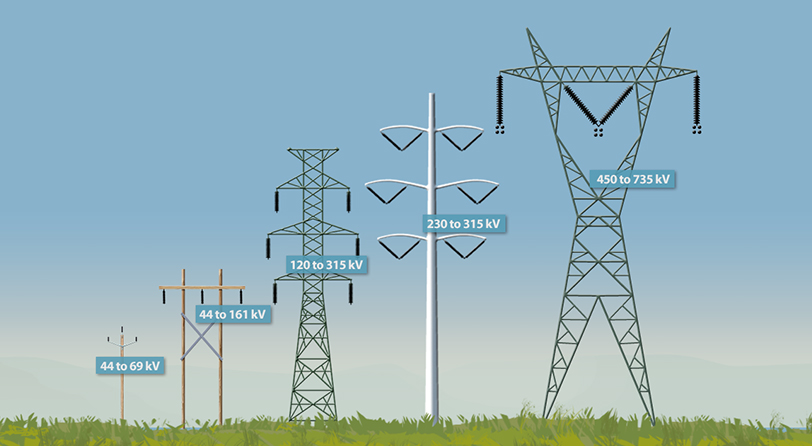
\includegraphics[width=\linewidth]{images/hq_securite_1-filsdangereux-en1-reconnaitrelesfils_img4-en.jpg}
\caption*{\href{https://www.hydroquebec.com/safety/transmission-lines/understand-transmission-lines.html}{\underline{Source}}}
\end{figure}
\column{0.45\textwidth}
\begin{figure}
\centering
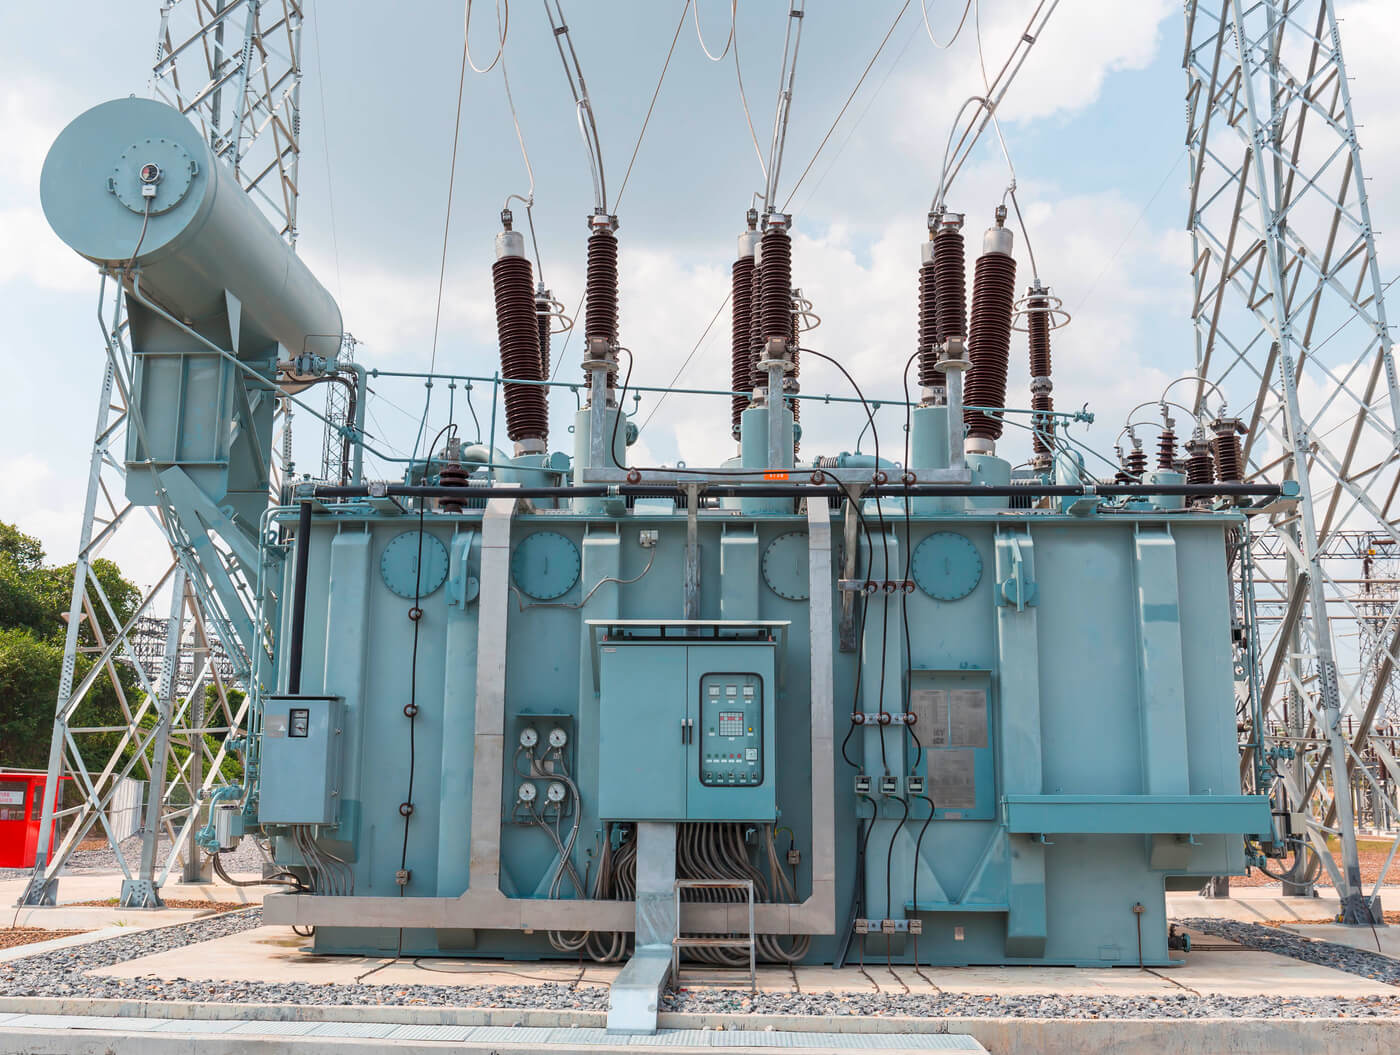
\includegraphics[width=0.9\linewidth]{images/What_Specifically_is_a_Power_Transformer.jpeg}
\caption*{\href{https://www.bbntimes.com/society/common-reasons-for-use-power-transformers-in-residential-areas}{\underline{Source}}}
\end{figure}
\end{columns}
\end{frame}

\begin{frame}
{Tens/hundreds of power plants + a myriad of distributed energy sources}
\begin{columns}
\column{0.5\textwidth}
\begin{figure}
\centering
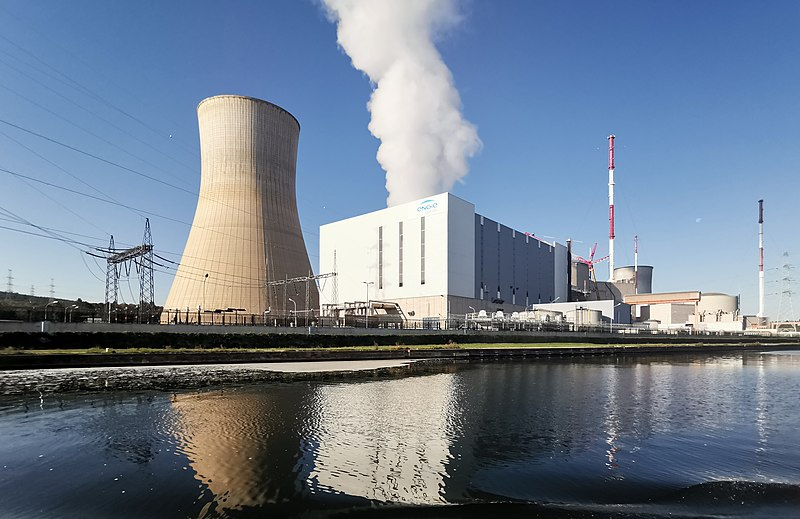
\includegraphics[width=0.9\linewidth]{images/Tihange_Nuclear_Power_Station.jpg}
\caption*{\small{Source: Wikipedia}}
\end{figure}
\column{0.5\textwidth}
\begin{figure}
\centering
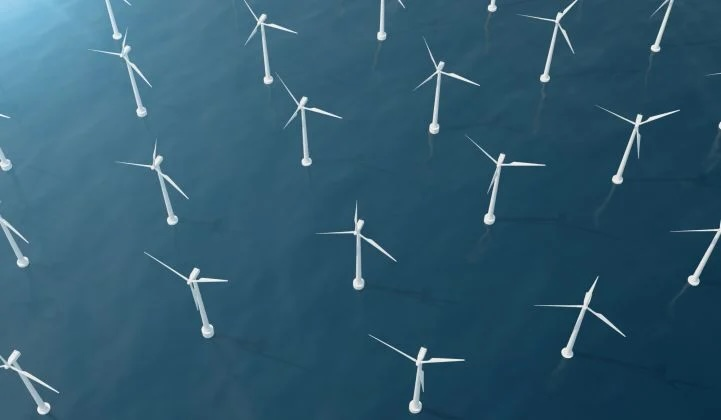
\includegraphics[width=0.9\linewidth]{images/Offshore_Wind_Aerial_XL_721_420_80_s_c1.jpg}
\caption*{\href{https://www.greentechmedia.com/articles/read/another-major-oil-company-invests-in-clean-energy1}{\underline{Source}}}
\end{figure}
\end{columns}
\end{frame}

\begin{frame}
{Devices to (dis)connect elements: substations, circuit breakers, isolators}
\begin{figure}
\centering
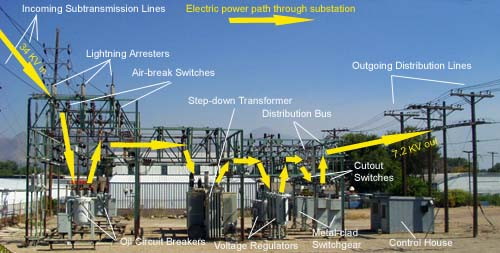
\includegraphics[width=0.7\linewidth]{images/substation_energy_flow.jpg}
\caption*{\href{https://www.osha.gov/etools/electric-power/illustrated-glossary/sub-station}{\underline{Source}}}
\end{figure}
\end{frame}

\begin{frame}
{Protection systems: to eliminate faults}
\begin{figure}
\centering
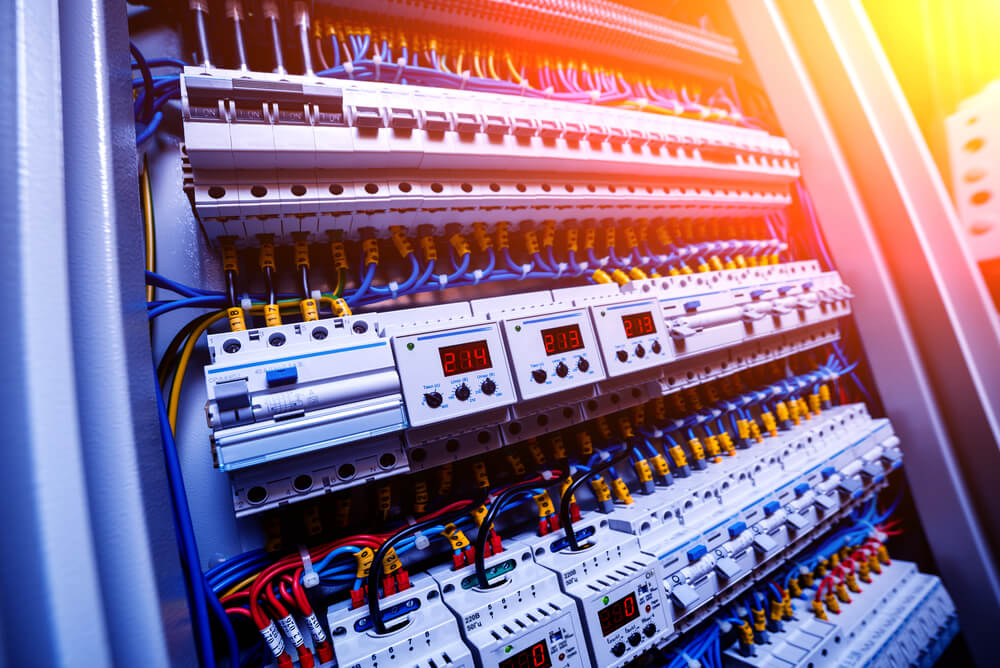
\includegraphics[width=0.5\linewidth]{images/shutterstock_679069147-1.jpg}
\caption*{\href{https://www.exa-ecs.com/courant-fort-quels-sont-les-composants-dune-armoire-electrique/}{\underline{Source}}}
\end{figure}
\end{frame}

\begin{frame}{Real-time measurements}

\begin{columns}
    \begin{column}{0.5\textwidth}
    Active and reactive power flows, voltage magnitudes, current magnitudes, energy meters, phasor measurement units
    \end{column}
    \begin{column}{0.45\textwidth}
      \begin{figure}
      \centering
      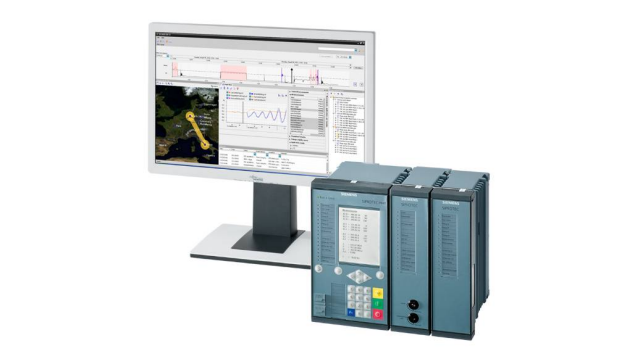
\includegraphics[width=\linewidth]{images/phasor-measurement-unit.png}
      \caption*{\href{https://new.siemens.com/global/en/products/energy/energy-automation-and-smart-grid/protection-relays-and-control/general-protection/phasor-measurement-unit-pmu.html}{\underline{Source}}}
      \end{figure}
    \end{column}
\end{columns}

\end{frame}

\begin{frame}{Controllers}
  \begin{columns}
    \begin{column}{0.4\textwidth}
      Distributed (e.g. in power plant) or centralized (control center)
    \end{column}
    \begin{column}{0.55\textwidth}
      \begin{figure}
      \centering
      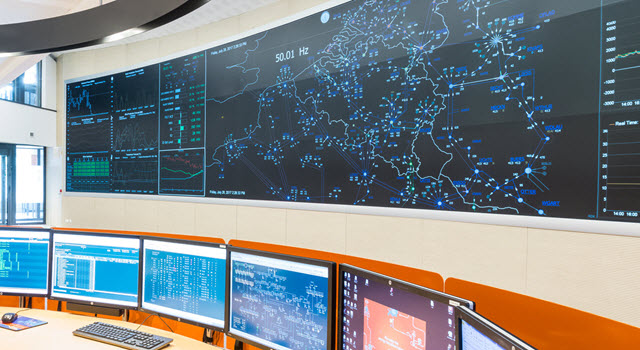
\includegraphics[width=\linewidth]{images/control-room-640x350-1.jpg}
      \caption*{\small{Source: \url{https://eliagrid-int.com/egi_projects/elia-national-control-centre-support/}}}
      \end{figure}
    \end{column}
    \end{columns}
\end{frame}

\begin{frame}
{Unlike most other complex systems built by man, power systems are exposed to external “aggressions”}
 Rain, wind, ice, storm, lightning, etc.
\begin{center}
\href{https://www.youtube.com/embed/bSSO5XT1k1I}{\underline{Example video}}
\end{center}
\end{frame}

\begin{frame}[allowframebreaks]{Low-probability but high-cost failures}
In spite of those disturbances, modern electric power systems are very reliable. Assume a duration of power supply interruption of 0.5 hour / year
\begin{center}
\textbf{availability =} (8760$-$0.5)/8760= \textbf{99.9\%} !
\end{center}
However, the cost of unserved energy is high
\begin{itemize}
\item average cost used by CREG (Belgian regulator) to estimate the impact of forced load curtailment: 8.3 k€/MWh (source: Bureau fédéral du plan)
\item varies with time of the day : between 6 and 9 k€/MWh
\item varies with type of consumer : 2.3 k€/MWh for domestic, much higher for industrial
\item even higher average cost considered elsewhere (e.g. 26 k€/MWh in France !)
\end{itemize}
Large-scale failures (blackouts) have tremendous societal consequences
\begin{itemize}
\item next two slides: examples of blackouts and their impacts
\end{itemize}
\end{frame}

\begin{frame}{USA-Canada blackout, August 2003}
\begin{columns}
\column{0.5\textwidth}
\begin{figure}
\centering
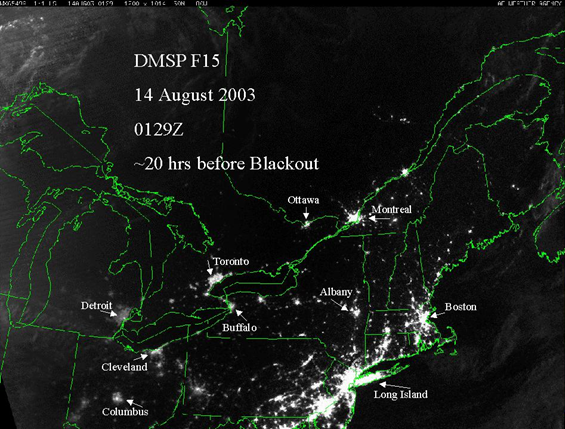
\includegraphics[width=0.7\linewidth]{images/pre_blackout_US.png}
\end{figure}
\begin{itemize}
\item 50 million people disconnected initially
\item 61 800 MW of load cut in USA \& Canada
\item cost in USA : 4 to 10 billion US \$
\end{itemize}
\column{0.5\textwidth}
\begin{figure}
\centering
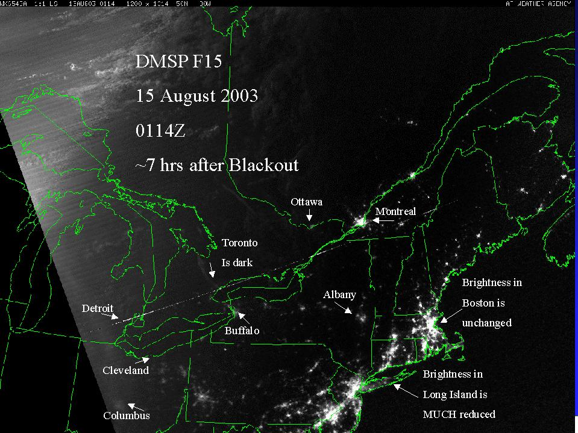
\includegraphics[width=0.7\linewidth]{images/post_blackout_US.png}
\begin{itemize}
\item Canada : 18.9 million working hours lost
\item 265 power plants shut down
\item restoration : from a few hours to 4 days
\end{itemize}
\end{figure}
\end{columns}

\footnotesize{Source : North American Electric Reliability Council (NERC)}
\end{frame}

\begin{frame}[allowframebreaks]{Italian blackout, September 2003}
\begin{itemize}
\item Cascade tripping of interconnection lines $\rightarrow$ separation of Italy from rest of UCTE system
\begin{figure}
\centering
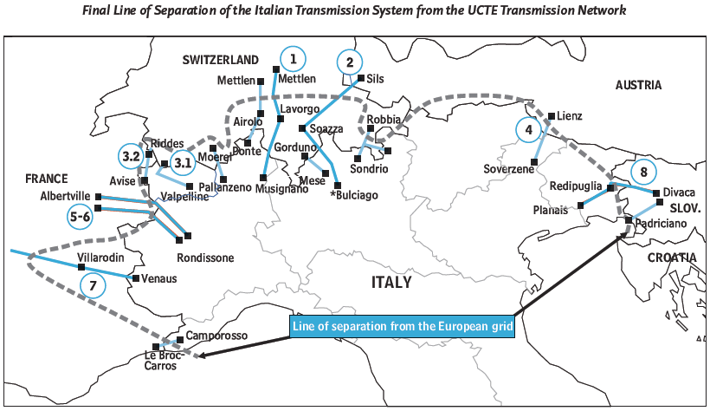
\includegraphics[width=0.5\linewidth]{images/blackout_italy.png}
\end{figure}
\item Deficit of 6.7 GW imported in Italian system $\rightarrow$ frequency to collapse in Italy
\item 340 power plants shut down, 55 million people disconnected initially - 27 GW lost (blackout occurred during night)
\item Estimated cost of disruption $\approx$ 139 million US \$
\item Restoration time: 15 hours
\end{itemize}
\vfill
\footnotesize{Source : Union for the Co-ordination of Transmission of Electricity (UCTE) which is now part of ENTSOe}
\end{frame}

\begin{frame}{Structure of electric network (case of Belgium)}

\begin{columns}
    \begin{column}{0.6\textwidth}
      \begin{figure}
      \centering
      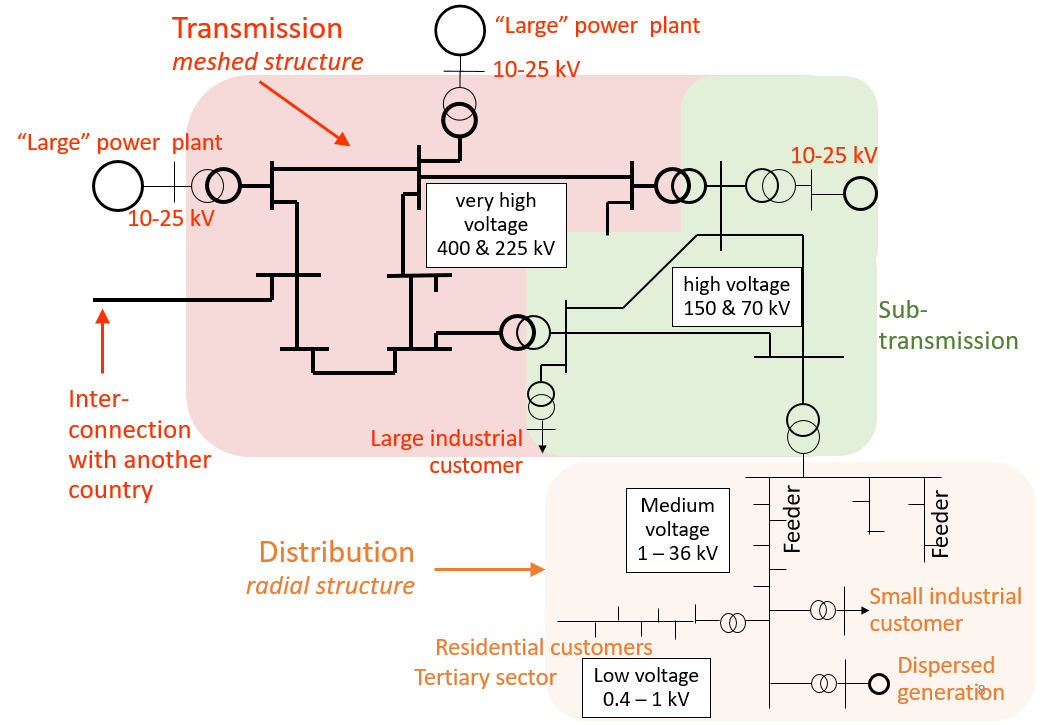
\includegraphics[width=\linewidth]{images/network_structure.png}
      \end{figure}
    \end{column}
    \begin{column}{0.35\textwidth}
      \footnotesize{In Belgium there are 30 and 36 kV underground cable networks, in Brussels and Antwerp areas. These are meshed and play the role of sub-transmission.}
    \end{column}
\end{columns}


\end{frame}

\begin{frame}{400 (and 220 kV) grid in Belgium and interconnections}
\begin{figure}
\centering
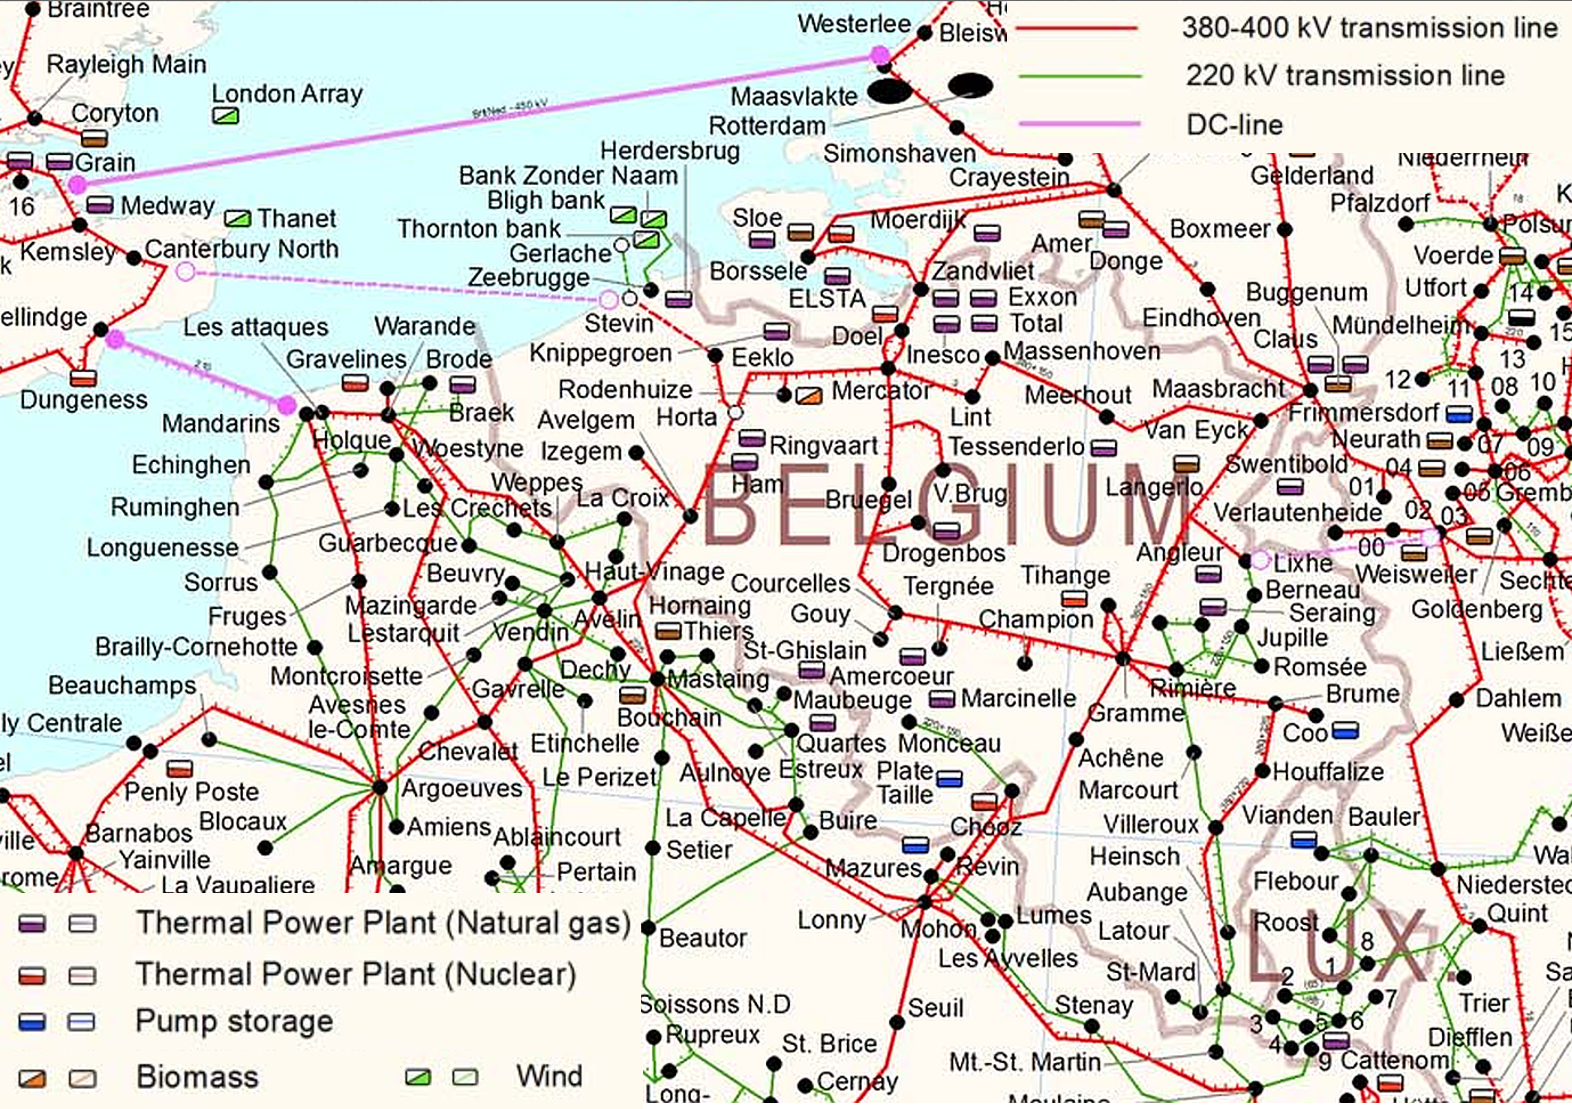
\includegraphics[width=0.6\linewidth]{images/intro_elia.png}
\end{figure}
\end{frame}

\begin{frame}{Flows on the belgian grid}
\begin{figure}
\centering
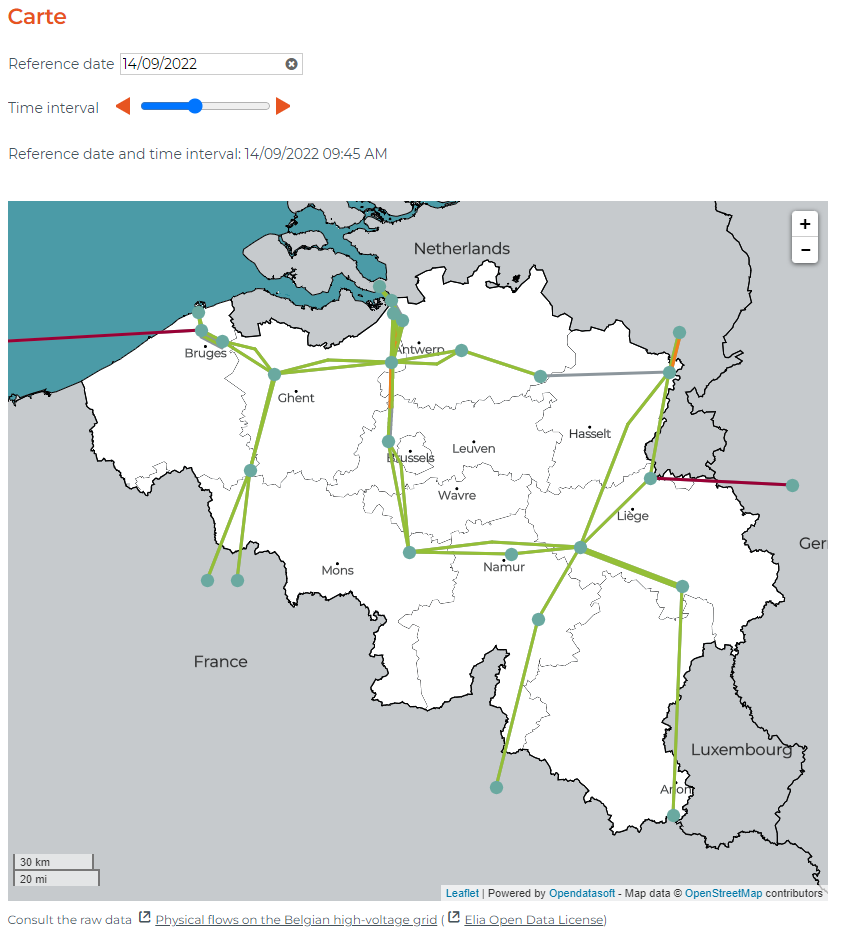
\includegraphics[width=0.4\linewidth]{images/20220914_ELIA_flows.png}
\end{figure}
\end{frame}

\begin{frame}{Length of network by voltage level and type in Belgium}
\begin{figure}
\centering
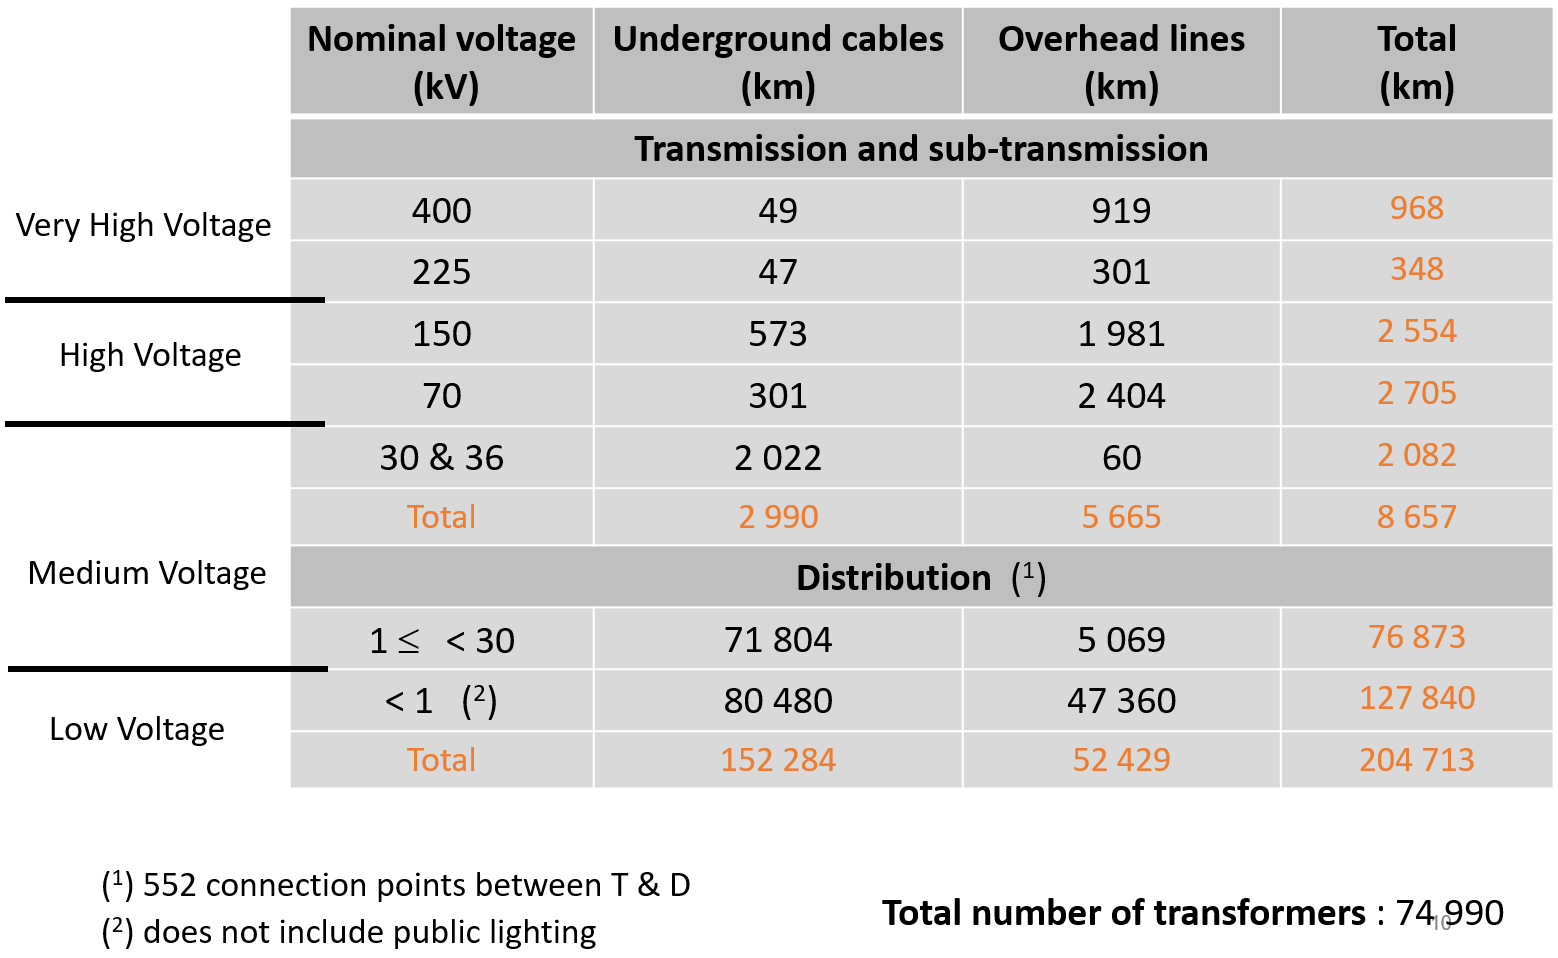
\includegraphics[width=0.6\linewidth]{images/stats_cables_and_lines_be.png}
\end{figure}
\vfill
\footnotesize{Source : SYNERGRID, as of December 2008}
\end{frame}


\section{Energy outlook for Belgium}

\begin{frame}
{Electrical energy balance over the year 2018 in Belgium}
\begin{figure}
\centering
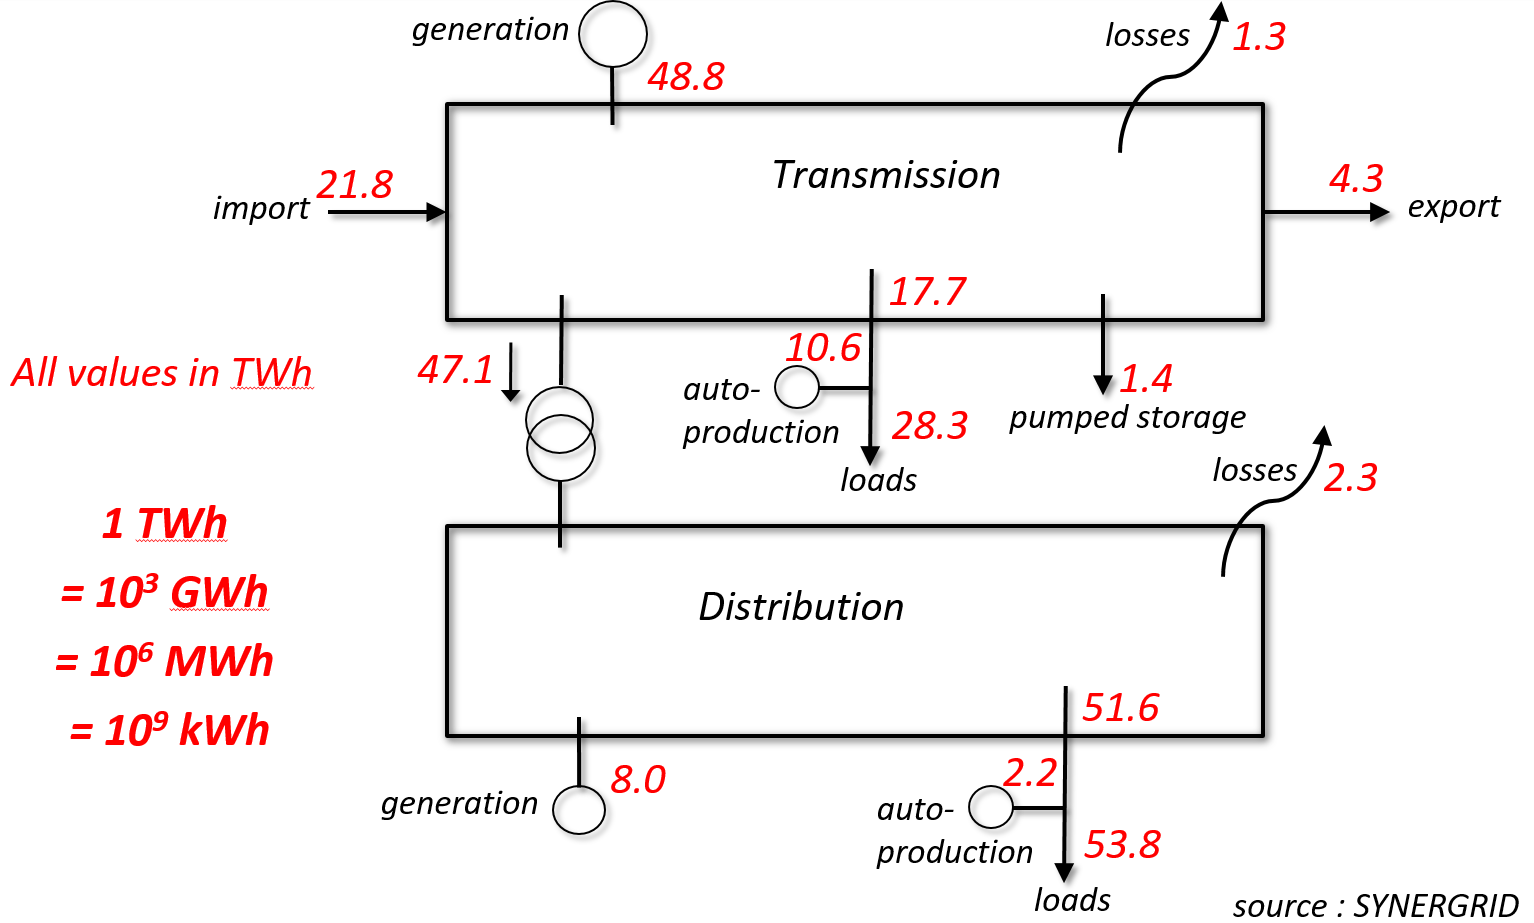
\includegraphics[width=\linewidth]{images/energy_balance_BE_2018.png}
\end{figure}
\end{frame}

\begin{frame}
{Network losses}
\begin{figure}
\centering
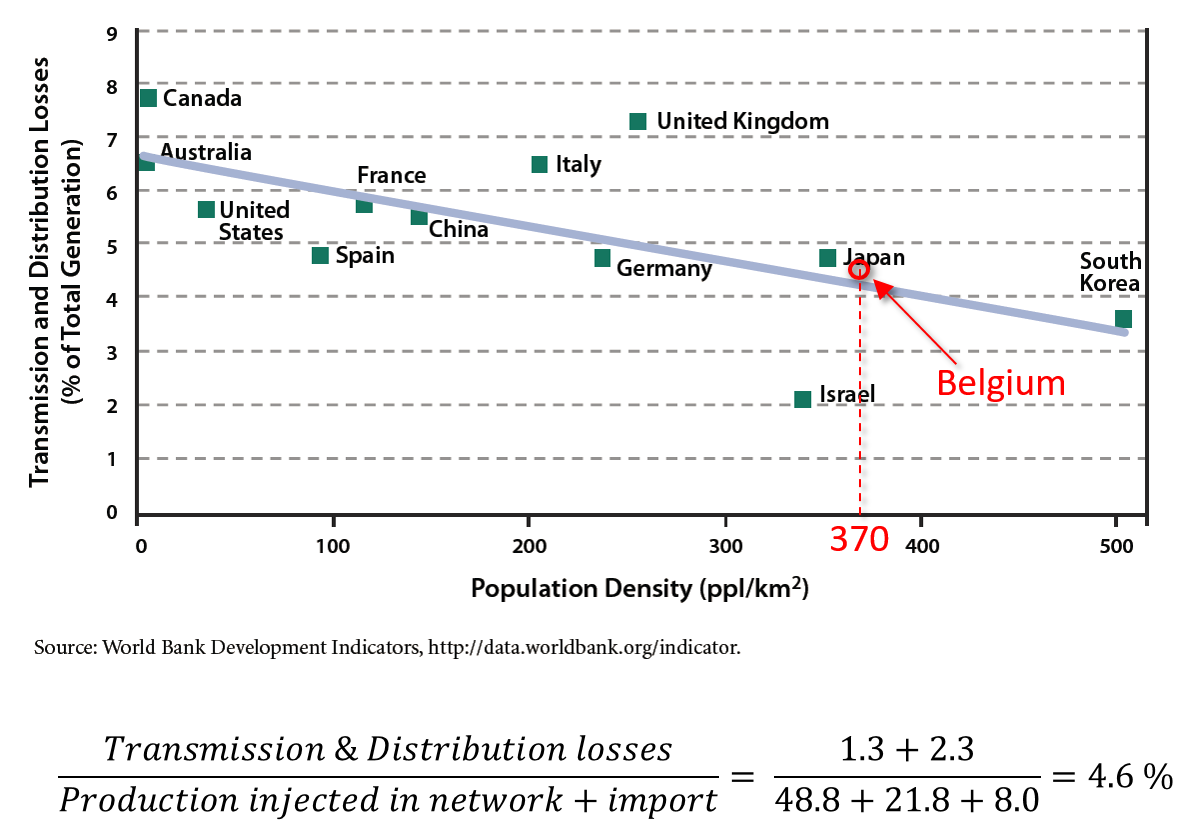
\includegraphics[width=0.9\linewidth]{images/network_losses_world.png}
\end{figure}
Transporting and distributing electrical energy is an industrial process with a relatively high efficiency
\end{frame}

\begin{frame}
{Consumption outlook}
\begin{figure}
\centering
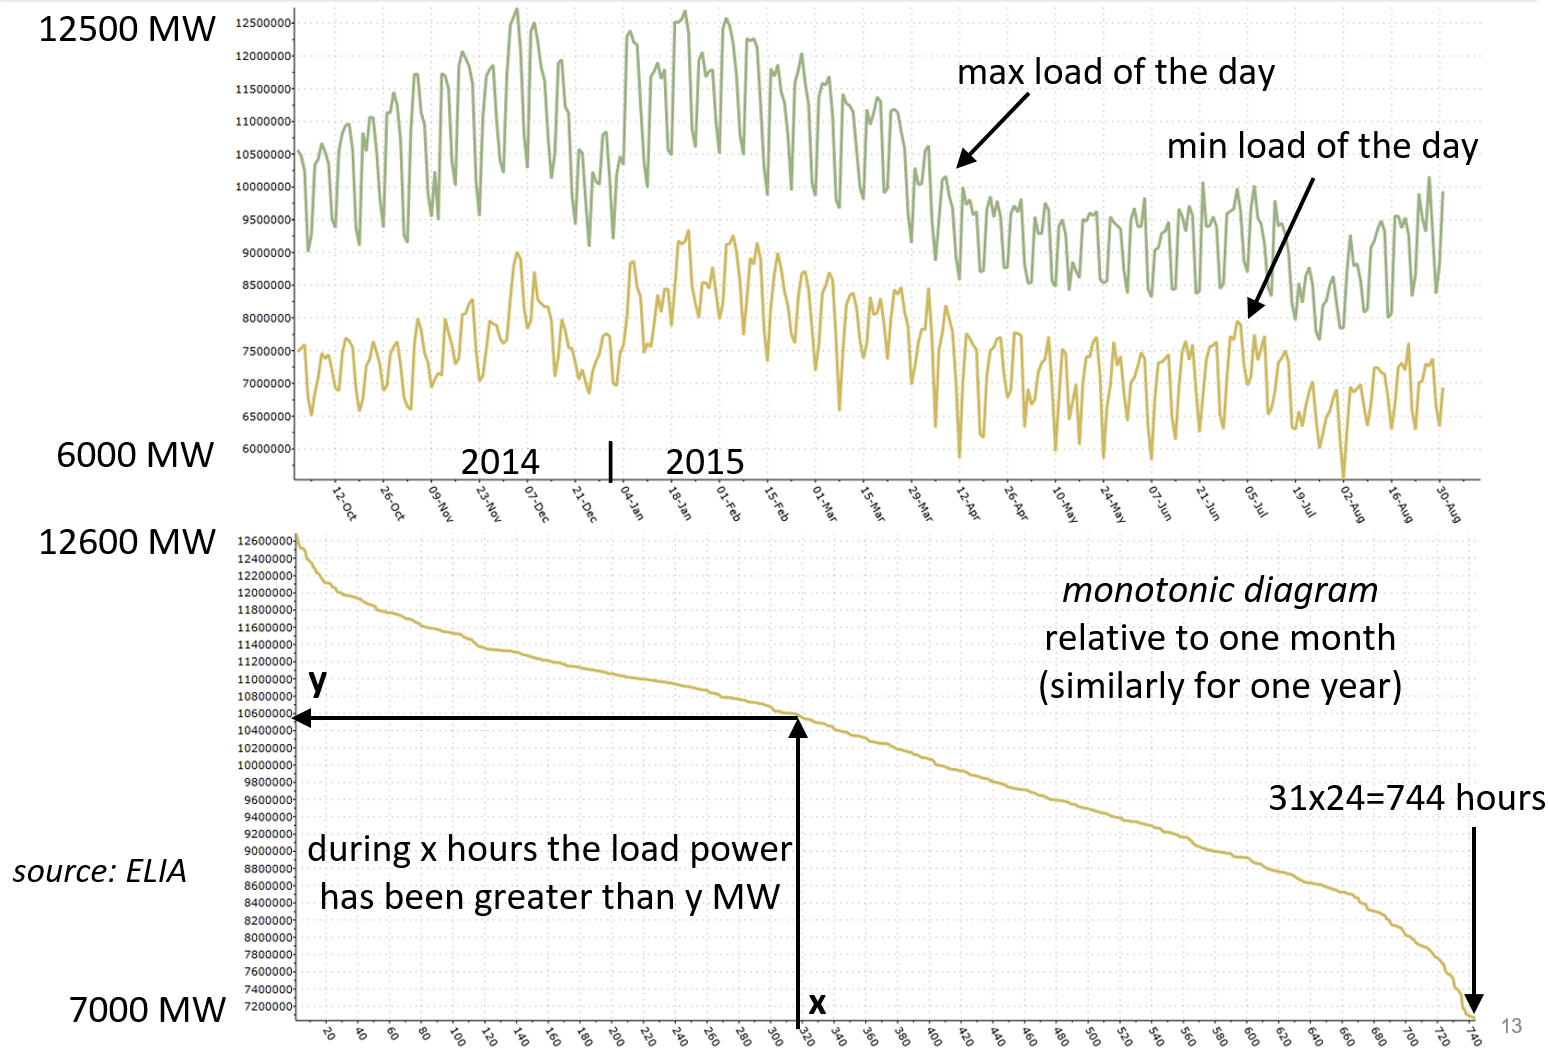
\includegraphics[width=\linewidth]{images/consumption_be.png}
\end{figure}
\end{frame}

\begin{frame}
\begin{figure}
\centering
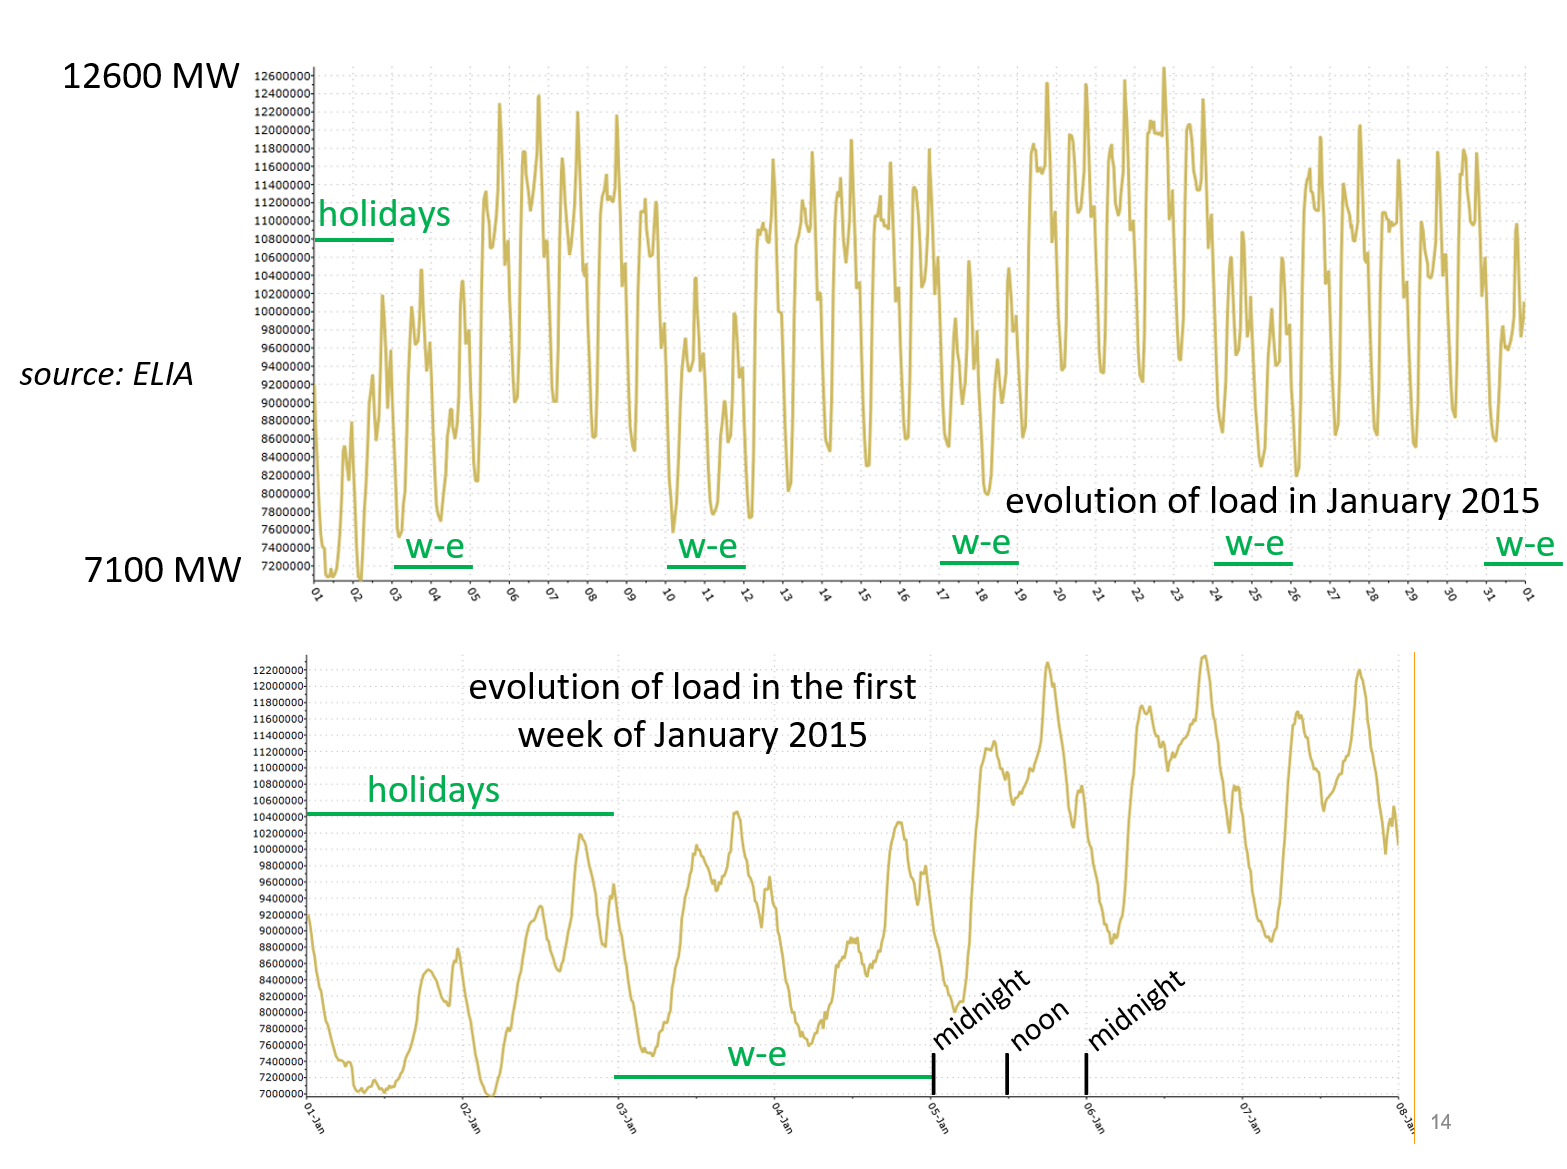
\includegraphics[width=\linewidth]{images/consumption_be_zoom.png}
\end{figure}
\end{frame}

\begin{frame}
{Peak load on some grids}
\begin{figure}
\centering
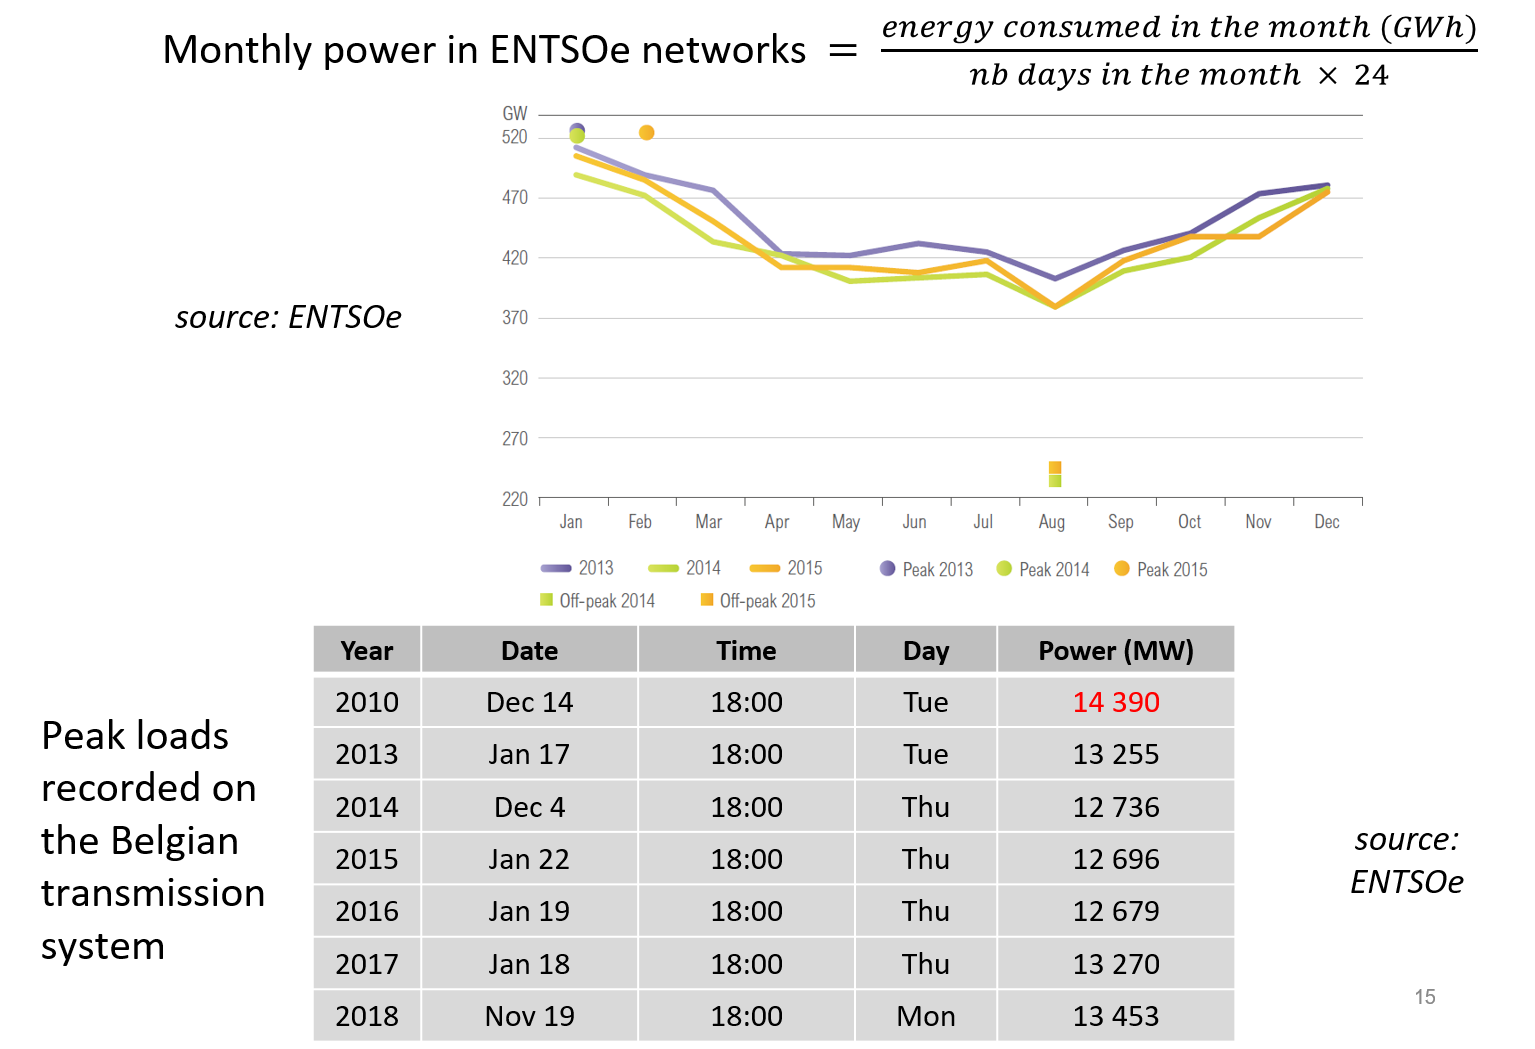
\includegraphics[width=\linewidth]{images/peaks_BE.png}
\end{figure}
\end{frame}

\begin{frame}
{Energy outlook for Belgium}
\end{frame}

\begin{frame}
{Sources of electrical energy in Belgium in 2018}
\begin{figure}
\centering
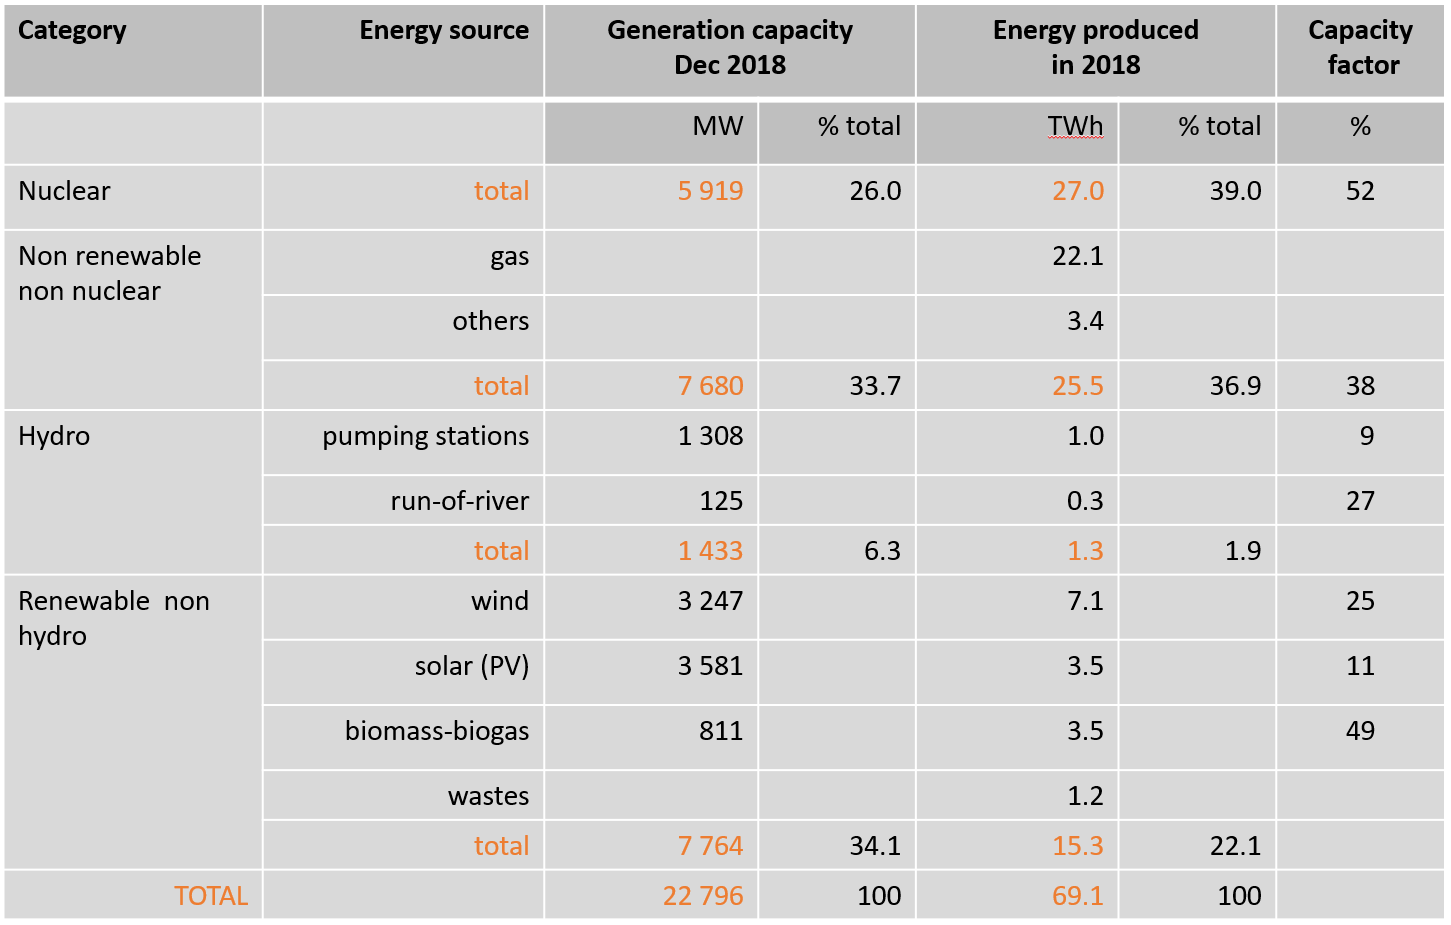
\includegraphics[width=\linewidth]{images/sources_BE.png}
\end{figure}
\vfill
\textbf{Exercise: let's update this table together.}
\vfill
\footnotesize{source : ENTSOE}
\end{frame}

\begin{frame}
{Comments}
\begin{itemize}
\item “Nuclear generation capacity” involves all units, even those temporarily shut down for technical reasons, or waiting for the decision to extend their lifetime
\item Gas power plants includes small CHP (Combined Heat Power) units
\item Same for biomass plants
\item Purposes of pumping storage :
\begin{itemize}
\item pumping : convert electrical energy into mechanical (potential) energy when demand is low compared to available generation (e.g. during night)
\item turbining : reverse operation when demand is high (e.g. at day peak) $rightarrow$ “peak shaving” and “valley filling” of daily load curve
\item efficiency of whole cycle $\approx$ 85 \%
\item usually profitable since cost of electricity higher when demand is high
\item fast reserve : a hydro unit can be started (resp. pumping stopped) quickly to replace a generation unit that is taken out of service
\item allows keeping base units (e.g. nuclear) in operation when load is very low
\end{itemize}
\end{itemize}
\begin{center}
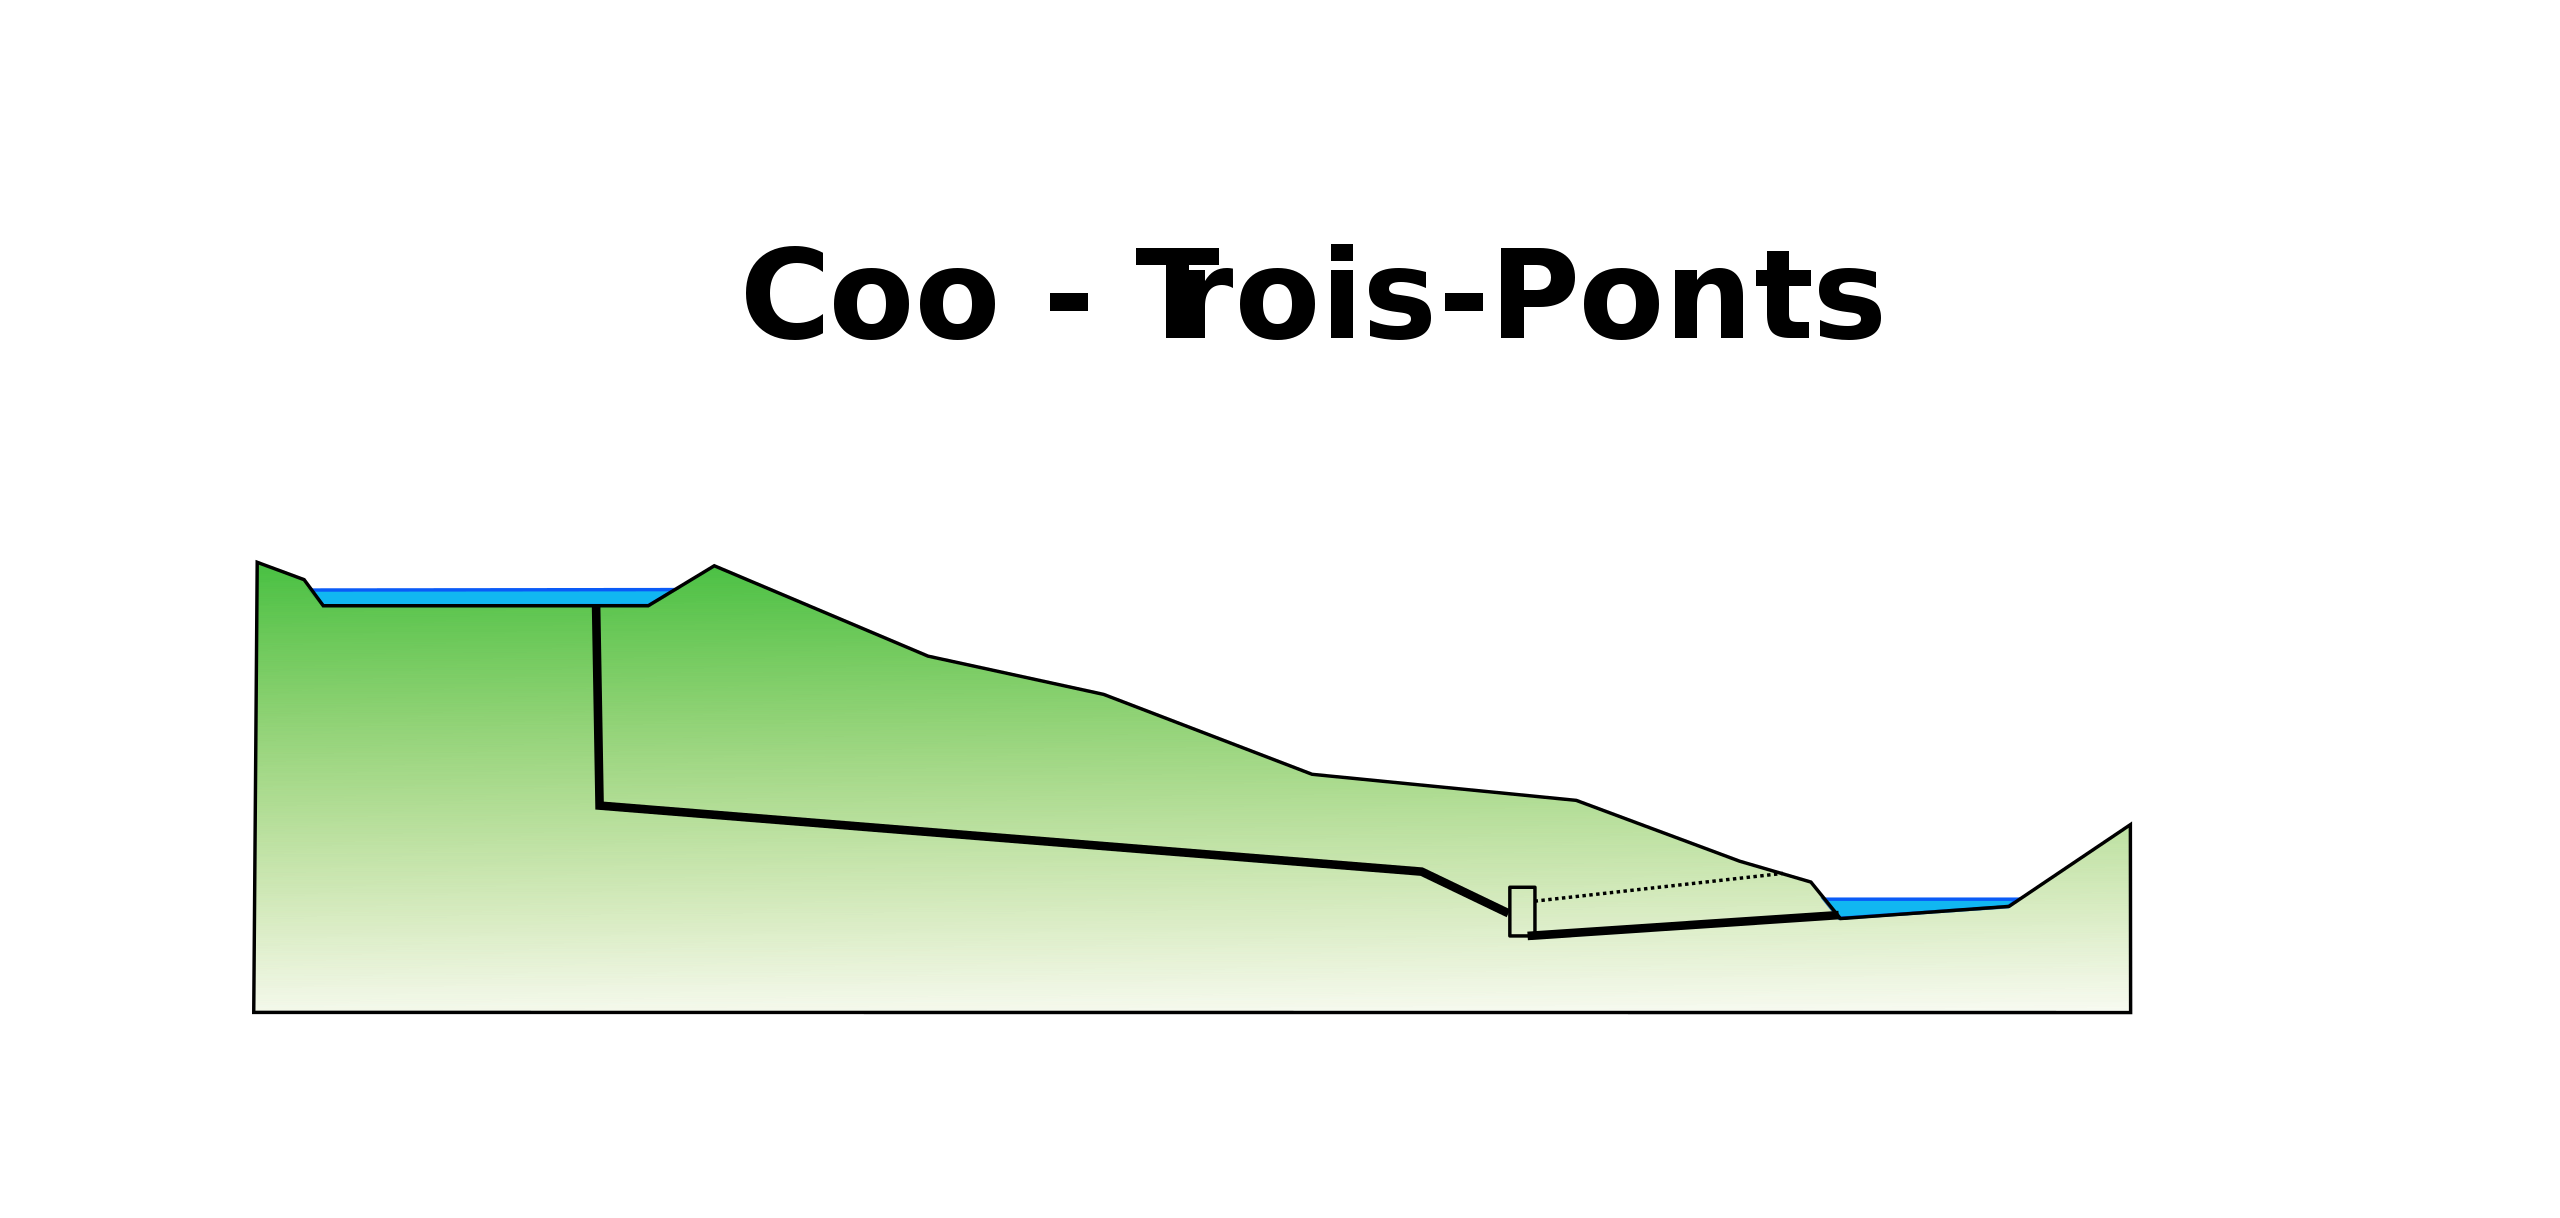
\includegraphics[width=0.4\linewidth]{images/Coo-Trois-Ponts.svg.png}
\end{center}
\end{frame}

\begin{frame}
{Comments: capacity factor}
\begin{itemize}
\item Capacity Factor:

%TODO generation capacity (MW)×365×24(h)
% energy produced in 1 year (MWh) 

\item usually close to 90 \% for nuclear, but some Belgian units have high unavailability
\item note the low value for solar energy!
\end{itemize}
\end{frame}

\begin{frame}
{Some trends in Belgium}
\begin{itemize}
\item Early retirement of gas power plants not enough competitive on electricity market, too expensive to maintain
\begin{itemize}
\item political decision to keep a “strategic reserve” !
\item \href{https://edfluminus.edf.com/edf/la-centrale-electrique-d-angleur}{Angleur}
\end{itemize}
\item \href{https://www.rtbf.be/info/regions/liege/detail_flemalle-fermeture-de-la-plus-grande-centrale-biomasse-de-wallonie-aux-awirs?id=10555470}{Biomass plant of "Les Awirs" just decommissioned.}
\item Natural hydro resources saturated in Belgium
\begin{itemize}
\item there are plans to expand the pumping storage
\item Coo power plant : currently $(3 \times 158 + 3 \times 230 =) $ 1164 MW installed capacity
\end{itemize}
\item Wind energy :
\begin{itemize}
\item public opposition to new on-shore wind farms (densely populated country !)
\item NIMBY attitude : Not In My BackYard
\end{itemize}
\end{itemize}
\end{frame}

\begin{frame}
{Some trends in Belgium (...)}
\begin{itemize}
\item off-shore wind farms have a higher capacity factor than on-shore ones: wind is more steady in the sea
\item Belgian off-shore wind farms in 2018 :
\begin{itemize}
\item 5 wind parks with an installed capacity of 1186 MW have produced 3,408 TWh
\item Capacity Factor = (3,408×10 
6
 )/(1186×365×24) = 32 \%
\end{itemize}
\item still a great potential for new off-shore wind farms :
\begin{itemize}
\item 3 under construction (+ 1076 MW) → 8 TWh production expected in 2020
\end{itemize}
\end{itemize}
\end{frame}


\section{Insight on renewable and dispersed generation}

\begin{frame}
{From large centralized to small dispersed power plants}
\begin{figure}
\centering
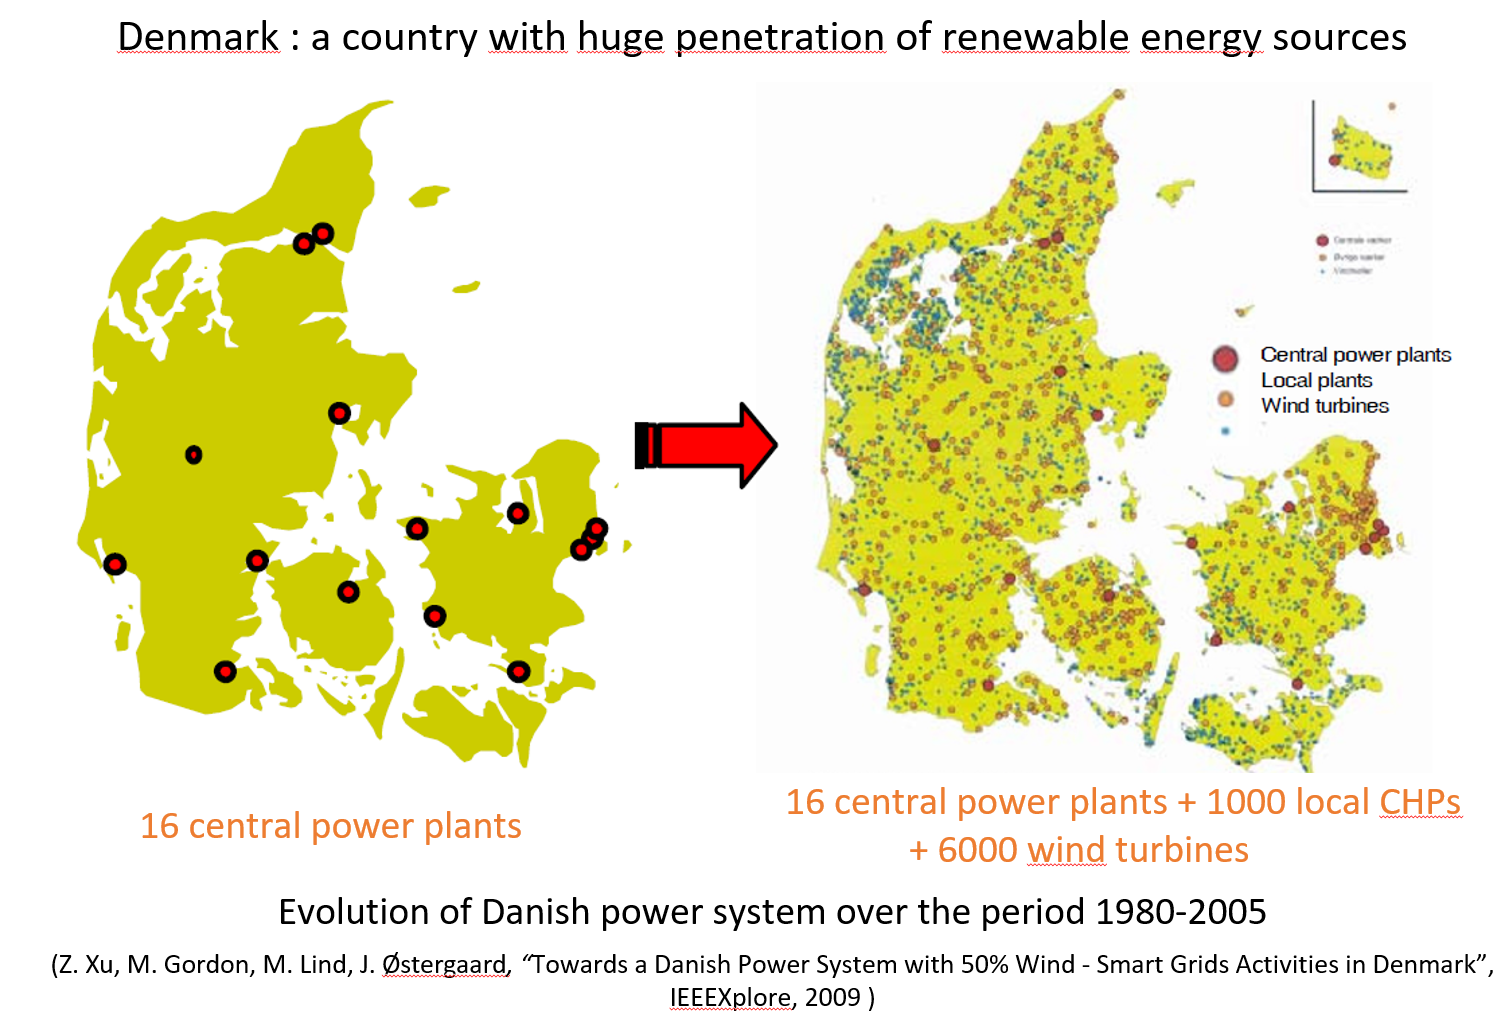
\includegraphics[width=\linewidth]{images/danemark_RES.png}
\end{figure}
\end{frame}

\begin{frame}
{Wind generation potential}
\url{https://globalwindatlas.info/}
\begin{figure}
\centering
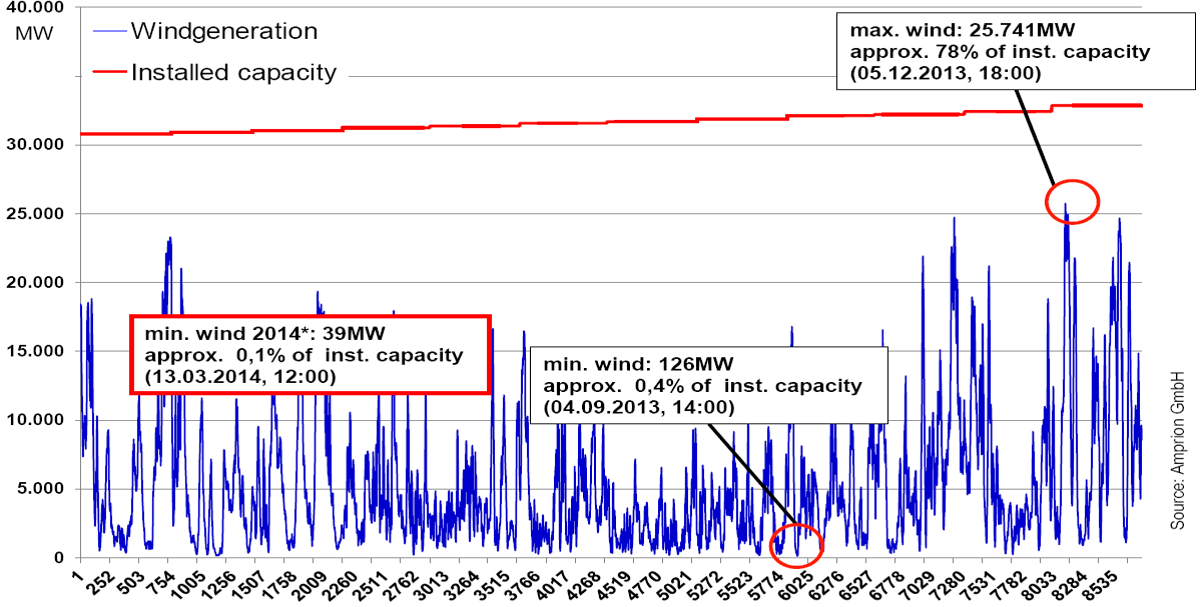
\includegraphics[width=\linewidth]{images/wind_gen_DE.png}
\caption*{Hour of the year 2013}
\end{figure}
\end{frame}

\begin{frame}{PV generation potential}
%\url{https://re.jrc.ec.europa.eu/pvg_download/map_index_c.html#!}
\begin{figure}
\centering
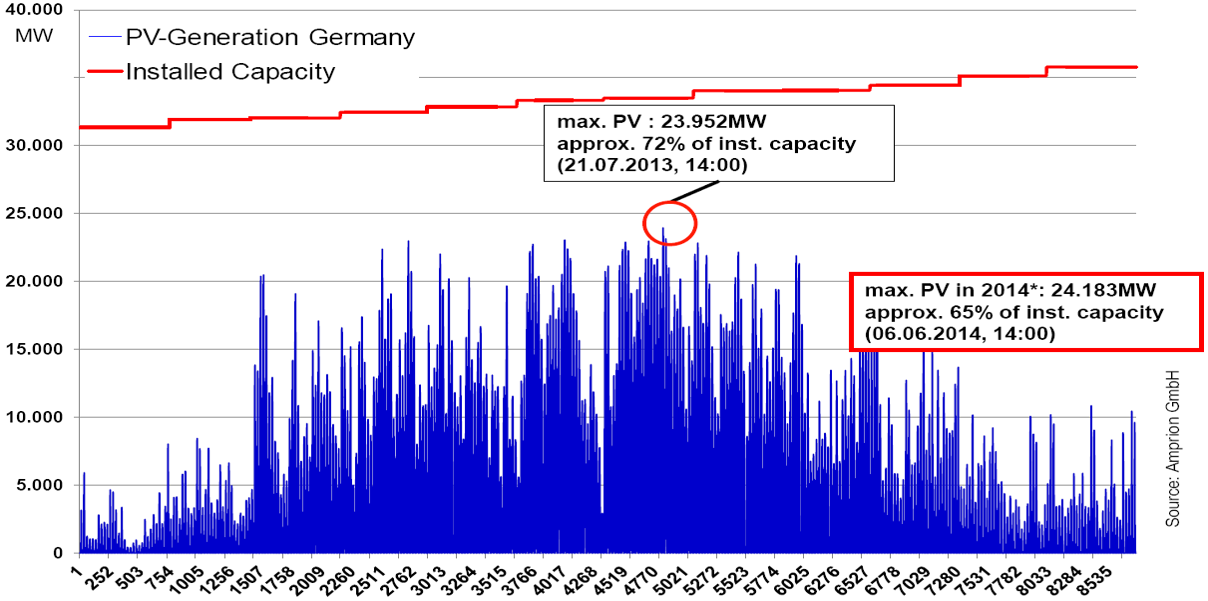
\includegraphics[width=\linewidth]{images/PV_gen_DE.png}
\caption*{Hour of the year 2013}
\end{figure}
\end{frame}

\section{The power balance problem}


\begin{frame}
{The power balance issue}
\begin{figure}
\centering
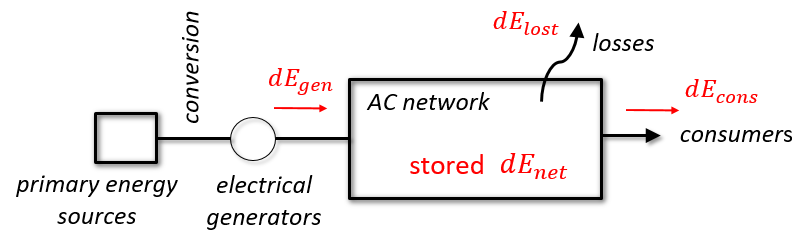
\includegraphics[width=0.8\linewidth]{images/power_balance.png}
\end{figure}
Conservation of Energy over an infinitesimal time dt:

$$dE_{gen} = dE_{cons} + dE_{lost} + dE_{net}$$Introducing the corresponding powers at time $t$:$$p_{gen}(t).dt = p_{cons}(t).dt + p_{lost}(t).dt + p_{net}(t).dt$$Hence$$p_{gen}(t) = p_{cons}(t) + p_{lost}(t) + p_{net}(t)$$

\end{frame}

\begin{frame}
$p_cons(t)$: The consumers decide how much power they want to consume !
\begin{itemize}
\item this demand fluctuates at any time
\end{itemize}
$p_lost(t)$: Losses mainly due to Joule effects → depend on currents in components
\begin{itemize}
\item kept as small as possible, not really controllable
\end{itemize}
\end{frame}

\begin{frame}
$p_net(t)$: Network elements which store electrical energy : inductors and capacitors
\begin{itemize}
\item In sinusoidal steady state, the power in an inductor (or a capacitor) reverts every quarter of a period, and is zero on the average
\begin{itemize}
\item in balanced three-phase operation, the sum of the powers in the inductors/capacitors of the three phases is zero at any time !
\item hence, electrical energy cannot be stored in the AC network
\end{itemize}
\item to be stored, electrical energy has to be converted into another form of energy
\begin{itemize}
\item mechanical: e.g. potential energy of water in the upper reservoir of a pumping station, flywheels, etc.
\item chemical: batteries, but amounts of stored energy are still very small !! Really?
\item \href{https://en.wikipedia.org/wiki/Hornsdale_Power_Reserve}{Hornsdale Power Reserve}
\item \href{https://www.energy-storage.news/blogs/sponsored-ngks-nas-grid-scale-batteries-in-depth}{NGK's batteries}
\end{itemize}
\end{itemize}
\end{frame}

\begin{frame}
{Conclusion}
The variations of load power have to be compensated by the generators but the conversion (primary energy → electrical energy) is not instantaneous
\begin{itemize}
\item example: changing the flow of steam or water in a turbine takes a few seconds
\end{itemize}
Hence, an “energy buffer” is needed to quickly compensate power imbalances
\begin{itemize}
\item this is provided by the rotating masses of synchronous generators
\item a deficit (resp. excess) of generation wrt load results in a decrease (resp. increase) of speed of rotation speeds (and hence, frequency)
\item in a synchronous generator and its turbine, kinetic energy $\approx$ nominal power of the generator produced during 2 to 5 seconds
\item controlling the power balance in a power system without rotating machines (only power electronic interfaces) would be a challenge (still at research level) !
\end{itemize}
Larger variations in load (e.g. during the day) require starting up/shutting down power plants ahead of time
\end{frame}

\section{From DC to AC, large interconnections and the come-back of DC}

\begin{frame}
{Network: from early DC ...}
End of 19th century : Gramme, Edison devised the first generators, that produced Direct Current (DC) under relatively low voltages
Impossibility to transmit large powers with direct current:
\begin{itemize}
\item power=voltage×current
\begin{itemize}
\item if the voltage cannot be increased, the current must be
\item but power lost=resistance×current 
2
  → big waste of energy
\item and large sections of conductors required → expensive and heavy
\end{itemize}
\item Hard to interrupt a large DC current (no zero crossing), for instance after a short-circuit
\end{itemize}
\end{frame}

\begin{frame}
{Network: ... to present high-voltage AC}
Changing for Alternating Current (AC)
\begin{itemize}
\item voltage increased and lowered thanks to the transformer
\item standardized values of frequency : 50 and 60 Hz (other values used at a few places)
\end{itemize}
Larger nominal voltages have been used progressively
\begin{itemize}
\item up to 400 kV in Western Europe
\item up to 765 kV in North America
\item experimental lines at 1100 kV or 1200 kV (Kazakhstan, Japan, etc.)
\end{itemize}
\end{frame}

\begin{frame}
{Motivations for large interconnections}
\begin{itemize}
\item Mutual support between partners to face the loss of generation units
\item Each partner would have to set up a larger “reserve” if it would operate isolated
\item Larger diversity of energy sources available within the interconnection
\item Allows exploiting complementarity of nuclear, hydro and wind power plants
\item Allows partners to sell/buy energy, to create a large electricity market.
\end{itemize}
\end{frame}

\begin{frame}
{Constraints:}
\begin{itemize}
\item If one partner is unable to properly “contain” a major incident, the effects may propagate to the other partners’ networks
\item A transaction from one point to another cannot be forced to follow a “contractual” path; it distributes over parallel paths (“wheeling”) : see example on another slide.
\begin{itemize}
\item Partners not involved in the transaction undergo the effects of the power flow.
\end{itemize}
\item In large AC interconnections, there may be emergence of badly damped interarea electromechanical oscillations (frequency in the range 0.1 - 0.5 Hz)
\begin{itemize}
\item Rotors of synchronous generators in one area oscillate against the rotors of generators located in another area
\end{itemize}
\item It may not be possible to connect two networks with different power quality standards
\end{itemize}
\end{frame}

\begin{frame}
{European networks}
\begin{columns}
\column{0.5\textwidth}
ENTSOe :
European Network of Transmission System Operators
for electricity
\par\medskip
41 Transmission System Operators (TSOs) from 34 countries
\column{0.5\textwidth}
\begin{figure}
\centering
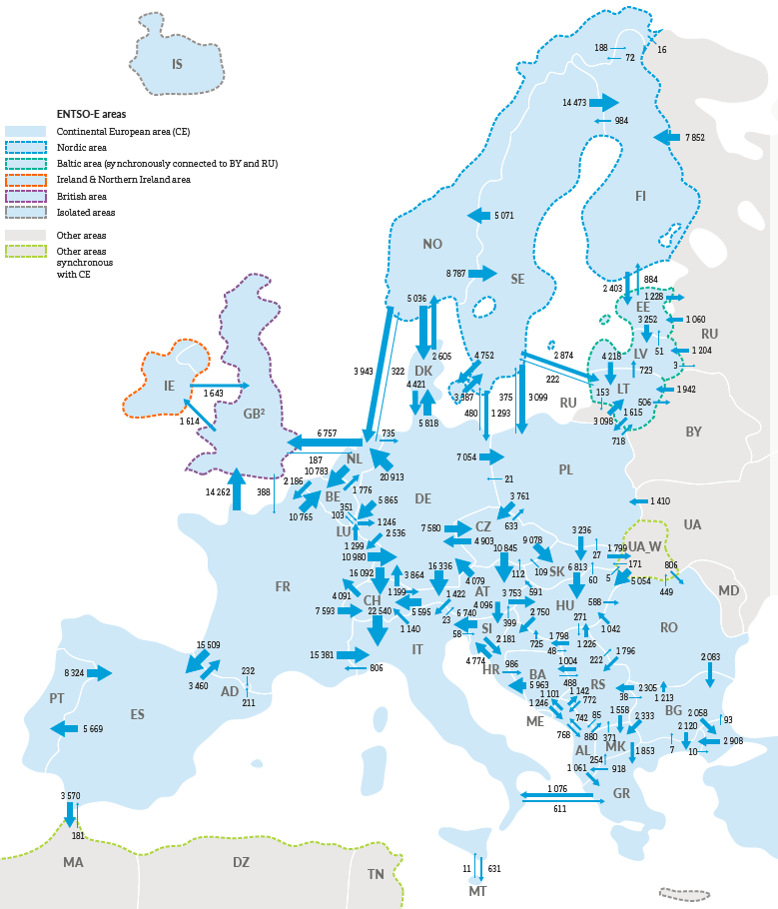
\includegraphics[width=\linewidth]{images/EU_net_flows.png}
\caption*{Energy flows in 2018 (in GWh)}
\end{figure}
\end{columns}
\end{frame}

\begin{frame}
{The synchronous grids of Europe}
\begin{figure}
\centering
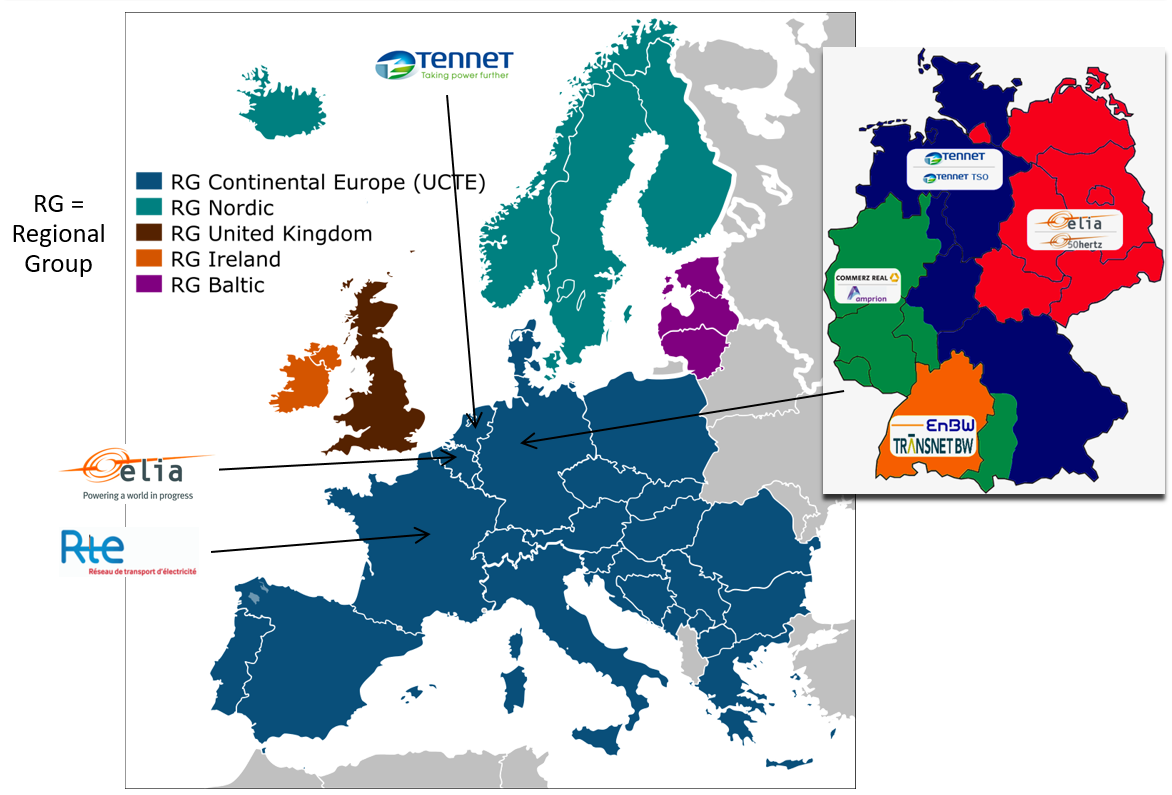
\includegraphics[width=\linewidth]{images/EU_TSOs.png}
\end{figure}
\vfill
\footnotesize{Source: ENTSOE}
\end{frame}

\begin{frame}
{Example of paths followed by power due to a transaction}
Paths taken by a production increment of 100 MW in Belgium
covered by a load increase of 100 MW in Italy (variation of losses neglected):
\begin{figure}
\centering
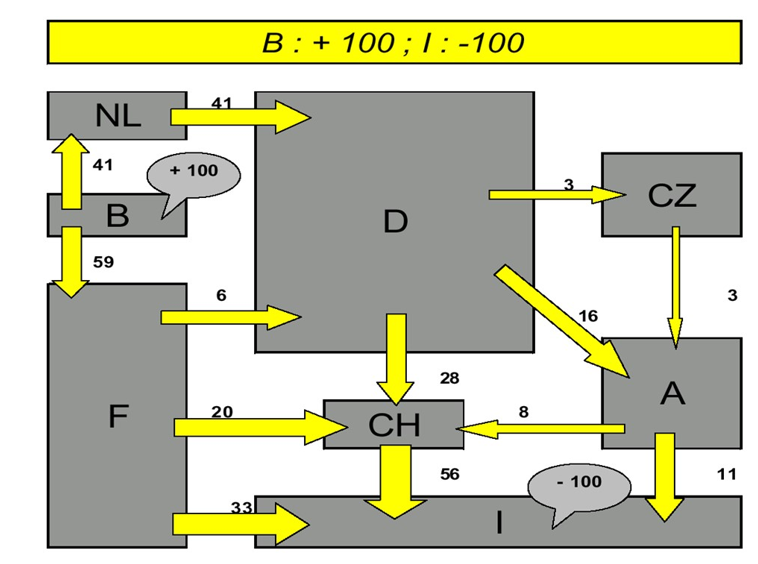
\includegraphics[width=0.5\linewidth]{images/EU_path_flows.png}
\end{figure}
\end{frame}

\begin{frame}
{The come-back of Direct Current}
Advances in power electronics → rectifiers and inverters able to carry larger currents through higher voltages → transmission applications made possible
\end{frame}

\begin{frame}
{Transmission over longer distances through overhead lines}
\begin{figure}
\centering
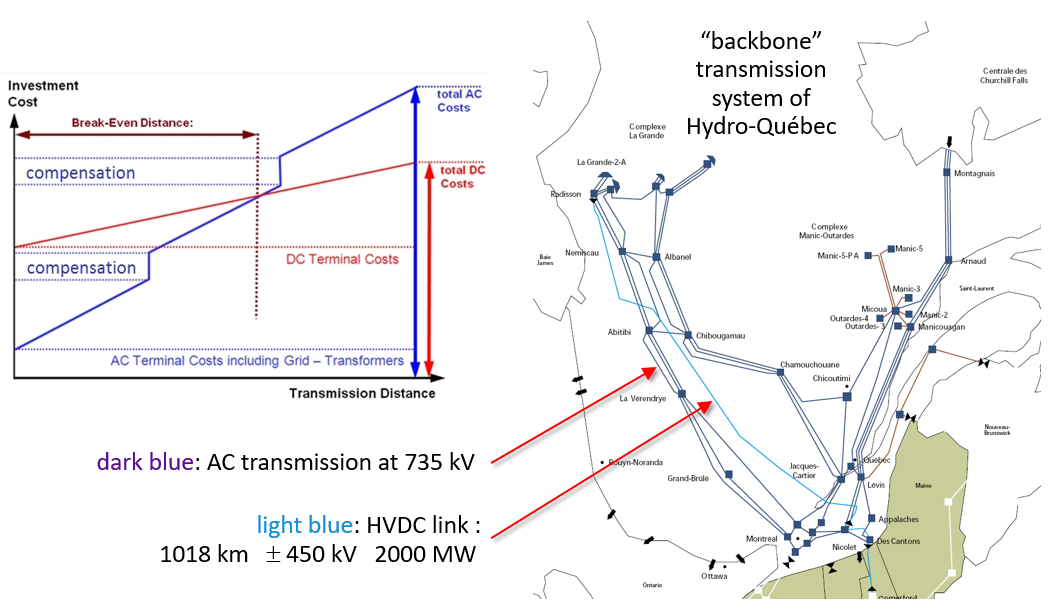
\includegraphics[width=0.9\linewidth]{images/DC_line.png}
\end{figure}
\end{frame}

\begin{frame}
{Transmission through submarine cables}
\begin{itemize}
\item DC more attractive than AC for distances above >= 50 km : owing to capacitive effects of AC cables
\item Existing links in Europe : see \href{https://www.elia.be/fr/donnees-de-reseau/transport/flux-physiques-sur-le-reseau-haute-tension-belge}{a previous slide}
\item Projects involving Belgium: Nemo with England, Alegro with Germany : see \href{https://www.elia.be/fr/donnees-de-reseau/transport/flux-physiques-sur-le-reseau-haute-tension-belge}{a previous slide}
\end{itemize}
\begin{columns}
\column{0.5\textwidth}
Connection of off-shore wind parks (source: ENTSOE, AC and DC connections of off-shore wind parks in North Sea to the grid of the Tennet German TSO, links under construction shown with dotted lines):
\column{0.5\textwidth}
\begin{figure}
\centering
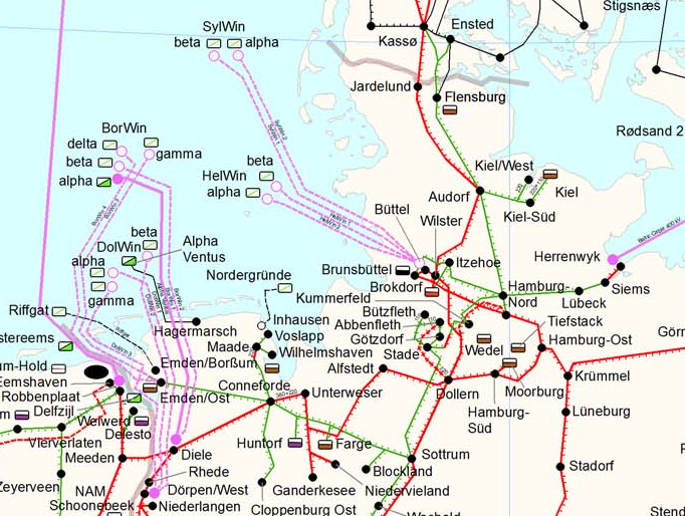
\includegraphics[width=\linewidth]{images/DC_cable.png}
\end{figure}
\end{columns}
\end{frame}

\begin{frame}
{Connection of AC networks with different frequencies or ...}
\begin{columns}
\column{0.5\textwidth}
\begin{itemize}
\item Two networks with different nominal frequencies
\begin{itemize}
\item connection of 50 and 60 Hz systems in Japan
\item connection of Brazil at 60 Hz with Argentina at 50 Hz
\end{itemize}
\item two networks that have the same nominal frequency but cannot be merged into a single C network, e.g. for stability reasons
\begin{itemize}
\item UCTE and Russian (IPS/UPS) system
\item Eastern - Western interconnections in North-America
\item Western Europe (see previous slides)
\end{itemize}
\end{itemize}
\column{0.5\textwidth}
\begin{figure}
\centering
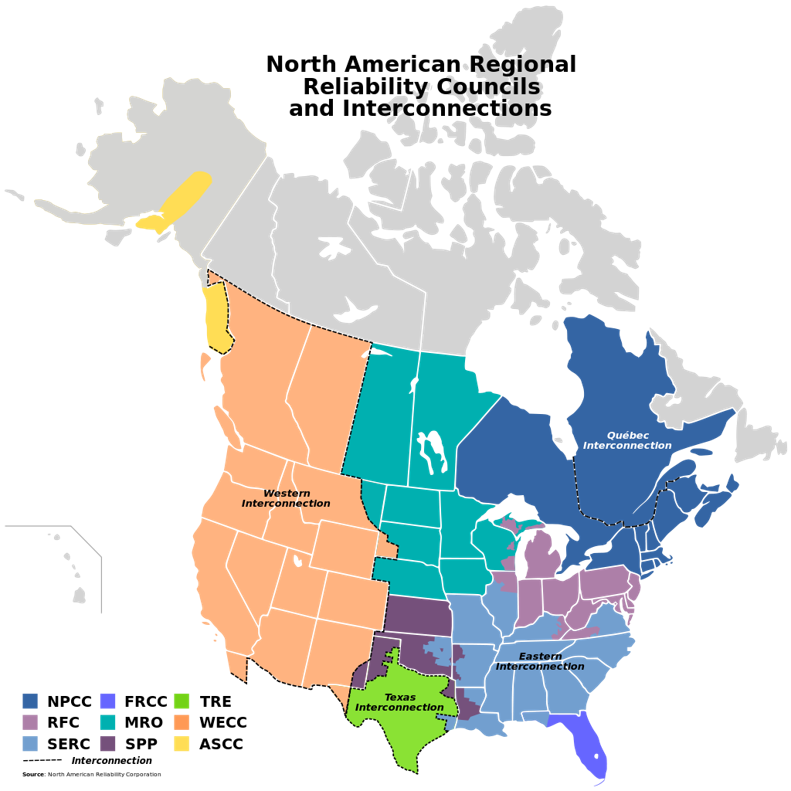
\includegraphics[width=\linewidth]{images/different_frequencies.png}
\end{figure}
\end{columns}
\end{frame}
